\documentclass[12pt]{kmutt}
\usepackage[left=40mm, right=20mm, top=30mm, bottom=20mm, includefoot=12.7mm, headheight=12.7mm]{geometry}
\usepackage{mathrsfs}
\usepackage{float}
%\usepackage{subfloat}
\usepackage{amsmath}
\usepackage{graphicx}
\usepackage{amsfonts}
\usepackage{afterpage}
\usepackage{amssymb}
%\usepackage{epsfig}
%\usepackage{subfigure}
\usepackage[usenames]{color}
\usepackage[labelfont=bf]{caption}
%\usepackage{caption}
\usepackage{subcaption}
\usepackage{cleveref}
\usepackage{braket}
\usepackage{afterpage}



\captionsetup{format = hang, labelsep=space}%This command is setting line of caption and removing colon from the picture captions.
\input{epsf.sty}
\linespread{1.5}
\def\thesection{\thechapter .\arabic{section}}
\setlength\parindent{0pt}

\begin{document}
    \newpage
    \thispagestyle{empty}
    \centerline{
\includegraphics[width=1.4in]{logo.jpg}}
\begin{center}
        {{\large\mbox BIREFRINGENT DIRAC FERMION IN ANISOTROPIC VELOCITY MODULATED GRAPHENE JUNCTION
}}\\
       \vspace*{6.75cm}
        {{\small\mbox   MR. EAKKARAT~~~PATTRAWUTTHIWONG}} \\
       {\small\vspace*{6.75cm}
               {\mbox{ A THESIS SUBMITTED IN PARTIAL FULFILLMENT OF THE REQUIREMENTS}\\
               FOR THE DEGREE OF MASTER OF SCIENCE  (PHYSICS) \\
               %DEPARTMENT OF PHYSICS \\
                FACULTY OF SCIENCE\\
                KING MONGKUT'S UNIVERSITY OF TECHNOLOGY THONBURI\\
               2020}
        }
\end{center}

    \newpage

    \pagenumbering{roman}
    \pagestyle{headings}
    \addtocontents{toc}{\contentsline{chapter}{}{PAGE}}
    \thispagestyle{empty}
    \begin{center}
    Electronic Transport of Dirac Fermion in Tilted Velocity Modulated Dirac Material Junction
    \\

    \vspace{1.5cm}

    Mr. Eakkarat    Pattrawutthiwong  B.Sc. (Applied Physics) \\

    \vspace{1.5cm}

    A Thesis Submitted in Partial Fulfillment of the Requirements for\\
    the Degree of Master of Science  (Physics) \\
    Faculty of Science \\
    King Mongkut's University of Technology Thonburi \\
    2020 \\
\end{center}

    \vspace{.3cm}\noindent Thesis Committee \vspace{1cm}

\noindent \begin{tabular}{cl}

    ...................................................................&   \hspace{0.3in} Chairman of Thesis Committee \\
    \noindent(Assoc. Prof. Bumned Soodchomshom , Ph.D.)  & \\ \\

    ...................................................................&   \hspace{0.3in} Member and Thesis Advisor\\
    (Asst. Prof. Watchara Liewrian, Ph.D.)  & \\ \\

    ...................................................................&   \hspace{0.3in} Member \\
    (Asst. Prof. Thana Sutthibutpong, Ph.D.)  & \\ \\

    ...................................................................&   \hspace{0.3in} Member\\
    (Tanapat Deesuwan, Ph.D.)  & \\ \\

    ...................................................................&   \hspace{0.3in} Member \\
    (Suwat Tangwancharoen, Ph.D.)  & \\ \\

\end{tabular}

\begin{center}
    Copyright reserved
\end{center}

    \newpage
    
   
    \, \quad \addcontentsline{toc}{chapter}{ABSTRACT IN THAI}
    \newpage

    \noindent 
{\begin{tabular}{ll} 
  Thesis Title &  Electronic Transport of Dirac Fermion in Tilted Velocity \\
               &  Modulated Dirac Material Junction \\
  Thesis Credits & 12 \\
  % Thesis Registration Credits & 1 \\
  Candidate & Mr. Eakkarat Pattrawutthiwong \\
  Thesis Advisor & Asst. Prof. Watchara Liewrian \\
  Program & Master of Science  \\
  Field of Study & Physics \\
  Department & Physics \\
  Faculty & Science \\
  Academic Year & 2020 \\
\end{tabular}}

\vspace{1cm}

\centerline{Abstract}

\vspace{1cm}

\noindent The ground state entanglement of the system, both in discrete-time and continuous-time cases, 
is quantified through the linear entropy. The result shows that the entanglement increases as the interaction 
between the particles increases in both time scales. It is also found that the strength of the harmonic potential 
affects the entanglement of the system. The different feature of the entanglement between continuous-time and 
discrete-time scales is that, for discrete-time entanglement, there is a cut-off condition. This condition implies that the 
system can never be in a maximally entangled state.
%%%%%%จากเปเปอร์

\vspace{1cm}


\noindent{Keywords\;:}  Continuous-Time/ Discrete-Time/ Entanglement


  

    \addcontentsline{toc}{chapter}{ABSTRACT IN ENGLISH}
    \newpage

    %
\vspace*{0.5cm} \centerline{\Large\bf ACKNOWLEDGEMENTS}
\vspace{1.5cm}
\noindent 
I would like to gratefully thank my advisor Asst. Prof. Watchara Liewrian for his support and guidance throughout my master's studies.
It was an invaluable experience working with him.
I would like to thank the faculty of science, King Mongkut's University of Technology Thonburi for granting me the graduated level scholarship,
and also the Thailand Center of Excellence in Physics for providing me the financial support on my research work. 
I appreciate the advices given by my colleagues and friends on both life and work.
Finally, I am grateful to my family, who encourage me during this challenging period of my life.

    %\addcontentsline{toc}{chapter}{ACKNOWLEDGMENTS}
    %\newpage

    \tableofcontents
    \addtocontents{toc}{\contentsline{chapter}{CONTENTS}{iv}}
    \newpage

    \listoffigures
    \addtocontents{toc}{\contentsline{chapter}{LIST OF FIGURES}{vi}}
    \addtocontents{lof}{\contentsline{chapter}{FIGURE}{PAGE}}
    \addtocontents{toc}{\contentsline{chapter}{}{}}
    \addtocontents{toc}{\contentsline{chapter}{CHAPTER}{}}
    \newpage

    \pagenumbering{arabic}
    \addtocontents{toc}{\protect\afterpage{~\hfill\textbf{PAGE}\par\medskip}}

    \kmuttchapter{INTRODUCTION}
\section{Background and motivation}
    Electronic transport in a two-dimensional (2D) system has been a popular topic in condensed matter physics since the first rise of Dirac material in 2004, known as graphene \cite{Zhang2004,Wehling2014}. 
    Their novel transport properties arise from linear energy dispersion, where charge carriers mimic massless Dirac fermion (MDF) \cite{CastroNeto2009}. 
    Graphene is one example of isotropic Dirac cone material, where energy dispersion around Dirac point has the same slope in $k_x$ and $k_y$ directions. 
    However, theoretical studies revealed that graphene Dirac cone could exist in the tilted and anisotropic manner by band engineering. 
    For example, by applying the periodic potential to graphene sheet, the anisotropy of Dirac cone can be tuned \cite{Park2008}. 
    The DFT calculation predicted that hydrogenated graphene exhibits Dirac material with tilted anisotropic Dirac cones \cite{Lu2016}. 
    The nitrogen line defects in graphene are also predicted to induce type-II over-tilted Dirac cone \cite{Zhang2017a}.\\

    In the last decade, great attention has been paid to investigate for new Dirac materials with anisotropic electronic properties. 
    For example, two-dimensional stacked layers of phosphorene known as black phosphorus \cite{Xia2014,Kim2015} and bulk structure of $\mathrm{SrMnBi_2}$ \cite{Park2011}. 
    Recently, borophene, a 2D allotrope of boron, has successfully grown on silver surfaces and predicted to host anisotropic tilted MDF \cite{Mannix2015a,Zhou2014}. 
    Also, it’s been reported that the anisotropy of high-Tc cuprate superconductors can be modulated by the hole doping \cite{Marino2019}.
    Anisotropic and tilt of Dirac material offer some novel electronic properties; for example, the superconducting gap has been predicted to be enhanced during the phase transition between type-I and type-II cone in Weyl semimetal \cite{Li2017a}. 
    In the context of transport properties, it has been demonstrated that electron optic behaviors with the opposite chiralities refracted into opposite directions, which may be useful for valley filtering \cite{Nguyen2018a}. 
    The tilted strength of a Weyl semimetal combined with the magnetic field effect considerably enhances the conductance gap \cite{Yesilyurt2017}. 
    The potential barrier and tilt effect is also predicted to induce the pseudo-magnetic field resulting in the asymmetric transmission \cite{Yesilyurt2017a}. 
    Therefore, it is beneficial to identify the tilted signatures of the Dirac cone to fine-tuning the electronic properties. 
    In fact, It has been shown that the anisotropic tilted Dirac cone in $\mathrm{\alpha-(BEDT-TTF)_2I_3}$ organic compounds can be measured by analyzing interlayer magnetoresistance \cite{Morinari2009}. 
    Recently, It has been also demonstrated that the Fano factor is sensitive to the tilt of the cone and can be used to verify the tilted signatures of material \cite{Trescher2015}.\\

    In this work, the tunneling properties of electrons across the mismatch of the tilted Dirac cone are investigated. 
    We first study the effect of the mismatch of the tilted Dirac cone on the electron transmission or resonance transmission in particular. 
    We then analyze the tunneling resonance condition of electron and propose a method to measure the tilted strength of the Dirac cone. 
    Moreover, we study the transmission under the influence of pseudo-magnetic field induced by the mismatch of the tilted Dirac cones
\section{Objectives}
    \begin{enumerate}
        \item Investigate the tunneling properties of Dirac electron through tilt-mismatch Dirac cone junctions.
        \item Determine the resonance condition of electron tunneling that can be used to identify the tilted strength of the Dirac cone.
        \item Design the tilt-mismatch Dirac material junction devices to indirectly measure the tilted strength of the Dirac cone.
        \item Study the tunneling behaviors of electron under the influence of pseudo magnetic effect induced by the tilt-mismatch Dirac cone.  
    \end{enumerate}
    

    %The electronic properties of material are defined by the ability of charge carriers to move throughout the crystal structures
    %The ability of charge carriers to tunnel throughout the material is defines by the crystal, electronic structures of their host material.
    %The electronic structure of material is critical, it defines the the ability of charge carriers to tunnel across the material.
    %Is has been proven that
    %The tunneling properties


    \kmuttchapter{THEORETICAL BACKGROUND}
Empty
    \kmuttchapter{MODEL AND METHOD}
In this work, the tunneling properties of electrons across the mismatch of the tilted Dirac cone are investigated.
We assume that the electron propagations are coherent and not affected by ohmic contact due to the heterogeneity of the junctions. 
The tunneling properties considered here are in low energy limit, in which the inter-valley scattering between $K$ and $K^\prime$ in the Brillouin zone is negligible \cite{Abergel2009}.
\section{Tilt-mismatch Dirac cone junction}
    The proposed structure is depicted in Fig. \ref{fig:transistor}, consisting of 2-dimensional Dirac material n-p-n heterojunctions with different tilted Dirac cones. 
    To achieve such a device structure, the top gate is placed in the middle region of length L to tune the Fermi energy level, which can be realized by depositing Ti/Au using standard electron beam lithography \cite{Huard2007}.
    Electrostatic doping using the ionic-liquid gate also has been demonstrated, which enhanced the carrier mobility \cite{Perera2013}. 
    For the barrier profile, we use rectangular potential barrier $U(x) = U[\Theta(x)-\Theta(x-L)]$.
    \begin{figure}[H]
        \centering
        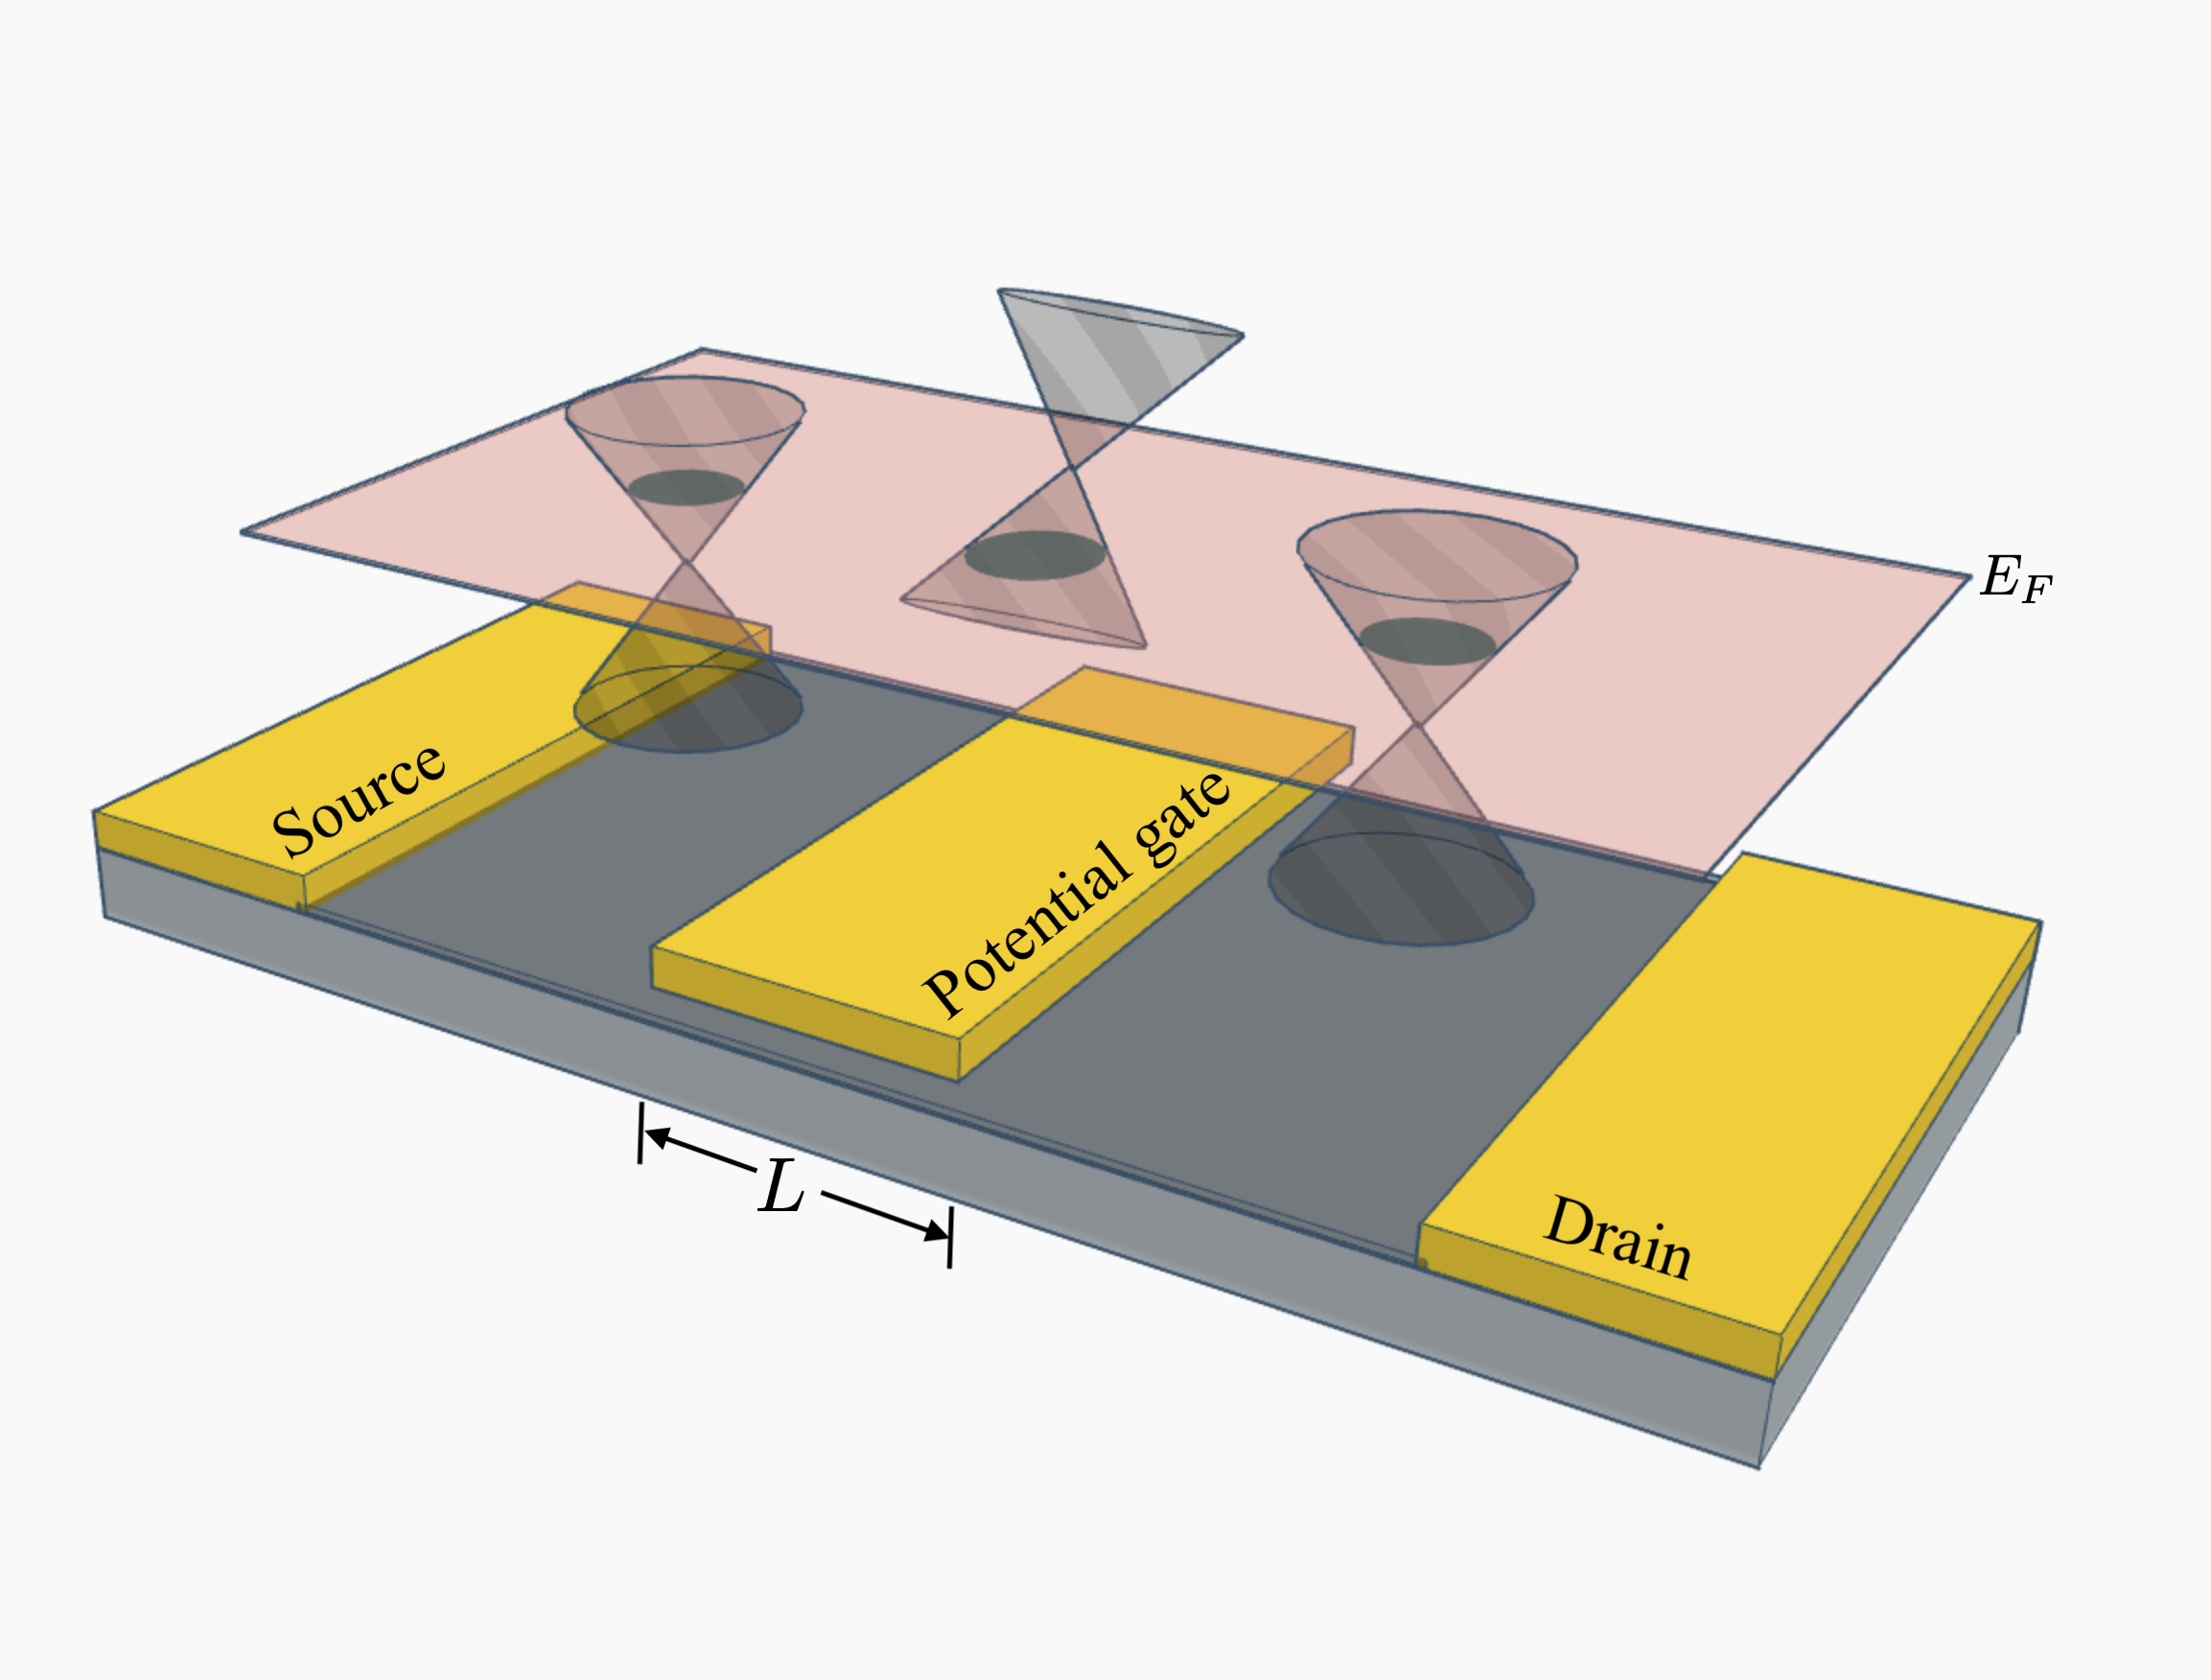
\includegraphics[width=0.6\linewidth]{fig/Transistor.png}
        \caption{Schematic illustration of Dirac material n-p-n heterojunctions with the mismatch of Dirac cone. 
                    The position of Fermi energy level $E_F$ can be controlled by tuning the voltage through potential gate of length $L$.}
        \label{fig:transistor}
    \end{figure}

\section{Transmission probability of electron in tilted Dirac cone}
    The wave function of Dirac electron in general Dirac materials can be obtain by solving the eigenvalue problem.
    Since the low-energy quasiparticles in Dirac material mimic relativistic particle, it can be described by effective massless Dirac Hamiltonian
    \begin{align} \label{eq:Hamiltonian}
        \hat{H} = \hbar (v_F \sigma \cdot k + w \sigma_0 \cdot k) + U \sigma_0
    \end{align}
    where U is barrier height, $v_F=10^6\ \mathrm{ms^{-1}}$ is Fermi velocity, $k=(k_x,k_y)$ is wave vector in the x-y plane, 
    $\sigma=(\sigma_x,\sigma_y)$ is Pauli matrices, $\sigma_0$ is a $2\times2$ identity matrix, 
    and $w=(w_x,w_y)$ is the parameter with the dimension of velocity denoting the tilt of Dirac cone.
    By solving Eq. \ref{eq:Hamiltonian}, we obtain the wave function for each region as follows
    \begin{equation}
    \begin{aligned}
        \psi_1 &= 
        \begin{cases}
            e^{ik_xx} +re^{-ik_xx} \ &, x<0\\
            s(e^{ik_xx}e^{i\phi} +re^{-ik_xx}e^{-i\phi}) \ &, x < 0
        \end{cases}\\
        \psi_2 &=
        \begin{cases}
            ae^{iq_xx} +be^{-iq_xx} \ &, 0\leq x<L\\
            s^\prime(ae^{iq_xx}e^{i\theta} -be^{-iq_xx}e^{-i\theta} )\  &, 0\leq x<L
        \end{cases}\\
        \psi_3 &=
        \begin{cases}
            te^{ik_xx}\ & ,x\geq L\\
            ste^{ik_xx}e^{i\phi}\ & ,x\geq L
        \end{cases}\\
    \end{aligned}
    \end{equation}
    The transmission coefficient $t$ can be obtained by considering the continuity of the wave function at the boundaries $x = 0$ and $x=L$
    \begin{equation} \label{eq:boundary condition}
        \begin{aligned}
            -a-b+r &= -1\\
            -sr e^{-i \phi }-s' \left(a e^{i \theta }-b e^{-i \theta }\right) &= -se^{i \phi }\\
            a e^{i L q_x}+b e^{-i L q_x}-t e^{i k_x L}&=0\\
            s' \left(a e^{i \theta +i L q_x}-b e^{-i \theta -i L q_x}\right)-s t e^{i k_x L+i \phi }&=0\\
        \end{aligned}
    \end{equation}
    It is easier to solve for $t$ using Cramer's rule. First put Eq. \ref{eq:boundary condition} into a matrix form, 
    where each column from left to right contain the factor of the coefficient $r, a, b,$ and $t$ respectively.
    \begin{equation}
        \mathrm{M_1}=
            \begin{pmatrix}
                1 & -1 & -1 & 0 \\
                -s e^{-i \phi } & -s'e^{i \theta } & e^{-i \theta } s' & 0 \\
                0 & e^{i L q_x} & e^{-i L q_x} & -e^{i k_x L} \\
                0 & s' e^{i \theta +i L q_x} & -s' e^{-i \theta -i L q_x} & -s e^{i k_x L+i \phi } \\
            \end{pmatrix}
    \end{equation}
    Then, replace the column $t$ with the factor on the right hand side of Eq. \ref{eq:boundary condition}
    \begin{equation}
        \mathrm{M_2}=
            \begin{pmatrix}
                1 & -1 & -1 & -1 \\
                -s e^{-i \phi } & -s'e^{i \theta }  & e^{-i \theta } s' & -s e^{i \phi } \\
                0 & e^{i L q_x} & e^{-i L q_x} & 0 \\
                0 & s_p e^{i \theta +i L q_x} & -s' e^{-i \theta -i L q_x} & 0 \\
            \end{pmatrix}
    \end{equation}
    The transmission coefficient $t$ can be obtain from $t = \det \mathrm{M_2}/ \det \mathrm{M_1}$
    \begin{equation}
        t = \frac{2 s s' \cos (\theta ) \cos (\phi ) (\sin (k_x L)+i \cos (k_x L))}
        {\sin (L q_x) \left(s^2-2 s s' \sin (\theta ) \sin (\phi )+s'^2\right)+2 i s s' \cos (\theta ) \cos (\phi ) \cos (L q_x)}
    \end{equation}
    The transmission probability can be obtained from $T = t^* t$
    \begin{equation} \label{eq:tp}
        T=\frac{\cos^2 \theta \cos^2 \phi}{\cos^2 (L q_x) \cos^2 \theta \cos^2 \phi + \sin^2 (Lq_x)(1-ss'\sin \theta \sin \phi )^2}
    \end{equation}
\section{The elliptic Fermi surface of tilted Dirac cone} \label{sec:elliptic fermi surface}
    When the Dirac cone is tilted, we obtain the elliptic Fermi surface in which the wavevector of electron is directional-dependent as shown in Fig. \ref{fig:elliptic fermi surface}.
    In other word, the length of vector $k$ varied as it rotate along the elliptic Fermi surface(dashed line).
    To understand relation between the electron wavevector and its incident angle $\phi$, we consider the elliptic equation where the major axis of the ellipse is in y-direction.
    \begin{figure}[H]
        \centering
        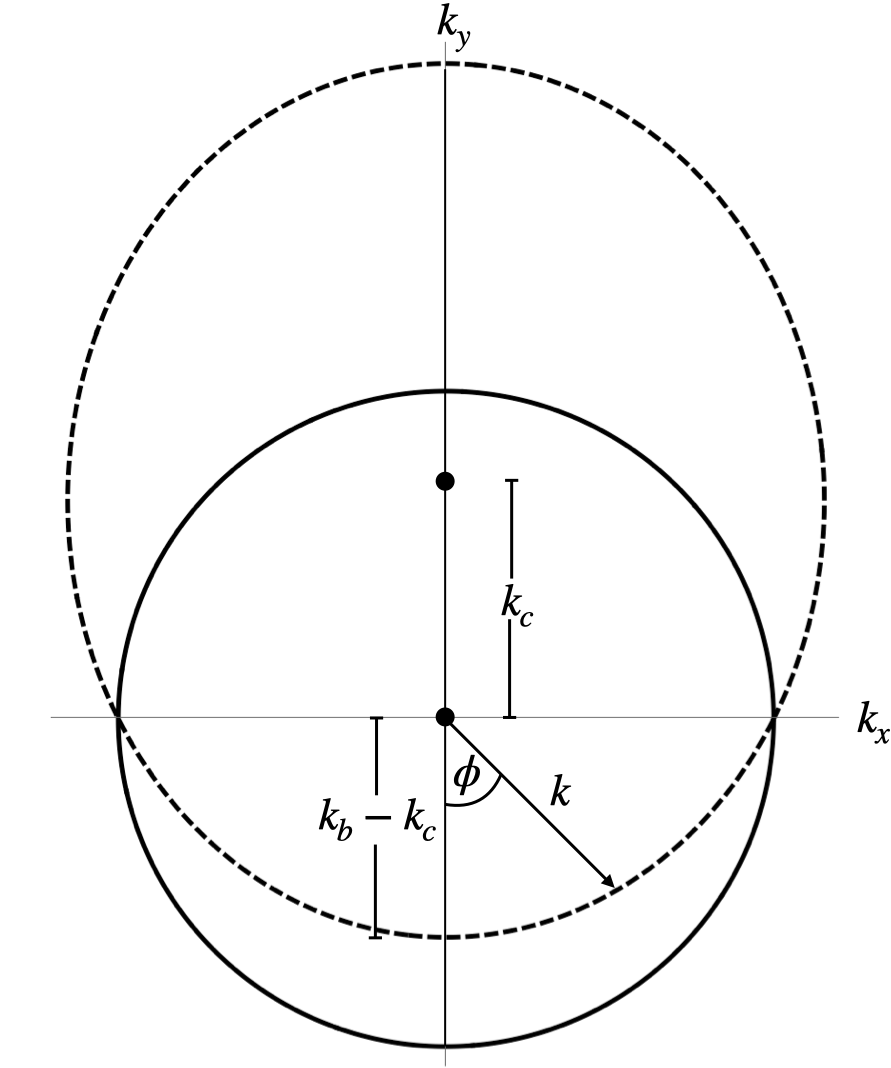
\includegraphics[width = 0.5\linewidth]{fig/elliptic fermi surface.png}
        \caption{The cross-sectional area of non-tilted and tilted Dirac cone with $w_0 = 0.5$ represented by solid and dashed line, respectively.}
        \label{fig:elliptic fermi surface}
    \end{figure}
    \begin{align} \label{eq:elliptic eq}
        \frac{k_x^2}{k_a^2} + \frac{k_y^2}{k_b^2} = 1
    \end{align}
    where $k_x = k\cos{\phi}$ and $k_y = k\sin{\phi} + k_c$. Multiply both side with $k_a^2 k_b^2$ and substituting $\cos^2{\phi} = 1 - \sin^2{\phi}$
    \begin{equation}
        \begin{aligned}
            k_b^2 k^2 -k_b^2 k^2 \sin^2{\phi} + k_a^2k^2 \sin^2{\phi}+2 k_a^2 k c \sin{\phi} +k_a^2 c^2)=k_a^2 k_b^2
        \end{aligned}
    \end{equation}
    Since $k_a = k_b \sqrt{1-w_0^2}$ and $k_c = k_b w_0$ where $w_0$ is eccentricity of the ellipse, we obtain
    \begin{equation}
        \begin{aligned}
            &k_b^2 k^2 - k_b^2 k^2 \sin^2{\phi} + k_b^2 (1-w_0^2)k^2 \sin^2{\phi}\\
            &+2 k_b^2 (1-w_0^2) k k_b w_0 \sin{\phi} +k_b^2 (1-w_0^2) k_b^2 w_0^2=k_b^2 (1-w_0^2) k_b^2\\
        \end{aligned}
    \end{equation}
    Multiplying both side with $-1/k_b^2$ and after some algebra, we obtain
    \begin{align} 
        k = \pm (k w_0 \sin{\phi} - k_b(1-w_0^2))
    \end{align}
    Since $k$ is nonnegative, we have to choose the solution such that $k$ is positive.
    Consider the case where $w_0 = 0$
    $$
    k = \pm (-k_b)
    $$
    We choose the negative solution in order for $k$ to be positive.
    \begin{equation}
    \begin{aligned} \label{eq:k vs phi}
        k &= -k w_0 \sin{\phi}+ k_b (1-w_0^2)\\
        k &= \frac{k_b(1-w_0^2)}{1+w_0 \sin{\phi}}
    \end{aligned}
    \end{equation}

\section{Angular dependent wavevector of tilted Dirac cone} \label{sec:k angular dependent k}
     
    We assume that the Dirac cone only tilted in y-direction. Therefore, the corresponding eigenenergy of Eq. \ref{eq:Hamiltonian} can be written as,
    \begin{align} \label{eq:eigenenergy}
        E_\eta=\hbar (\eta \sqrt{k_x^2 v_x^2+k_y^2 v_y^2 }+k_y w_y)+U
    \end{align}
    where $\eta$ is band index. Since the tilt of Dirac cone determines the shape of Fermi surface in which the wave vector $k$ is directional dependent. 
    In order to see the form of wave vector under the effect of tilted Dirac cone, Eq. \ref{eq:eigenenergy} can be rearranged to elliptic form as
    \begin{align}
        \frac{k_x^2}{k_a^2} + \frac{(k_y+k_c)^2}{k_b^2} = 1
    \end{align}
    where
    $$
    k_a = \frac{(E_F-U) v_y}{\hbar v_x \sqrt{(\eta^2 v_y^2 - w_y^2)} }, k_b = \frac{\eta v_y (E_F-U)}{\hbar (\eta^2 v_y^2 - w_y^2)},
    k_c = \frac{(E_F - U)w_y}{\hbar (\eta^2 v_y^2 - w_y^2)}
    $$
    We have, in section \ref{sec:elliptic fermi surface}, introduced the wavevector of electron as a function of incident angle $\phi$.
    We can substitute $k_b$ and $k_c$ to Eq. \ref{eq:k vs phi}, which gives
    \begin{align} \label{eq:k vs phi final}
        k = \frac{k_b(1-w_0^2)}{1+w_0 \sin{\phi}} = \frac{E_F - U}{\eta \hbar v_F (1+w_0 \sin{\phi})}
    \end{align}
    where
    \begin{equation} \label{3eq: tilted parameter}
        w_0 = \frac{k_c}{k_b} = \frac{(E_F - U)w_y}{\hbar (\eta^2 v_y^2 - w_y^2)} \frac{\hbar (\eta^2 v_y^2 - w_y^2)}{\eta v_y (E_F-U)} = \frac{w_y}{\eta v_F}
    \end{equation} 
    is tilted parameter and $\eta$ is band index indicating that the conduction and valence band always tilted in the opposite direction. 
    Eq. \ref{eq:k vs phi final} is the angular dependent wavevector outside the barrier as a function of incident angle $\phi$.
    Similarly, the wavevector inside the barrier region can be written as
    \begin{equation} \label{eq:q vs theta}
        q = \frac{E_F - U}{\eta \hbar v_F (1+w_0 \sin{\theta})}
    \end{equation}
    where $\theta$ is the refracted angle of electron inside the barrier. 
    This angle depends on the incident angle $\phi$, which can be obtained by considering the conservation of transverse wavevector
    \begin{equation} \label{eq:theta}
        \begin{aligned}
            q_y&=k_y\\
            q\sin{\theta} &= k \sin{\phi}\\
            \theta &= \sin^{-1}\left(\frac{k}{q}{\sin{\phi}}\right).\\
        \end{aligned}
    \end{equation}
    Substitute $\theta$ that we derived above to Eq. \ref{eq:q vs theta}, we obtain
    \begin{equation} \label{eq:q}
        q = \frac{E_F-U}{\hbar v_F s^{\prime}}+\frac{w_0 k_y}{s^{\prime}},
    \end{equation}
    and their x-component can be written as
    \begin{equation} \label{eq:qx}
        \begin{aligned}
        q_x &= \sqrt{q^2-q_y^2}\\
        q_x &= \sqrt{\left(\frac{E_F-U}{\hbar v_F}+w_0 k_y\right)^2-k_y^2}.\\
        \end{aligned}
    \end{equation}


    \kmuttchapter{RESULT AND DISCUSSION}
%section 1: Asymmetric tunneling
We start by investigating the tunneling properties of electron across tilted Dirac cone heterojunctions where we focus on how
the effect of the gate potential and tilt affect the electron transmission.  
%section 2: Measure the tilted strength 
%we focused on the tilted parameter $w_0$ since it is the parameter that determines the character of the Dirac cone.
Then, we demonstrate a method to measure the tilted strength of the Dirac cone by identifying the tunneling behavior.
%section 3 Pseudo magnetic field
Finally, we show that the transport behaviors of electron in tilted Dirac cone material are analogous to electron under
the influence of magnetic field. We also show the derivation of magnetic field strength as a function of gate potential and tilted parameter.


The calculation of transmission probability is carried out using Eq. \ref{eq:tp}
%In this study, we assumed that the system is in a condensed state, where the thermal noise can be neglected
\section{Angular dependent of transmission probability} \label{sec:asym}
    The transmission probabilities across the tilted Dirac cone heterojunctions under the variation of gate potential are presented in Fig. \ref{fig:asym}.
    The transmission profiles are symmetric in the case of $w_0 = 0$ regardless of the gate potential. 
    When the tilted parameter is non-zero, the transmission profiles are shifted along the direction of the tilt and consequently become asymmetric, where the magnitude of the shift depends on the tilted strength of the Dirac cone.
    However, the present of the tilt barely affects the tunneling profiles when the applied gate potential is close to the Fermi energy as shown in Fig. \ref{fig:asym2}.
    This is because the Fermi surface is small and the allowed wavevector states are narrowed. Therefore, electron propagations other than the normal incident are backscattered.\\
    
    Interestingly, when the applied gate voltage $U$ is larger than the Fermi energy $E_F$, the transmission profiles exhibit peak tunneling as shown in Fig. \ref{fig:asym3}-\subref{fig:asym4}.
    These kind of tunnelings are called resonant tunneling, which occurred when the condition $q_x L = n \pi$, $n = 0, \pm1,...$ in Eq. \ref{eq:tp} is met.
    %In addition, the normal incident perfect tunneling is not affected by the transverse tilted Dirac cone.
    
    \begin{figure}[H] %Asymmetric tunneling
        \centering
        \begin{subfigure}[b]{0.3\linewidth}
            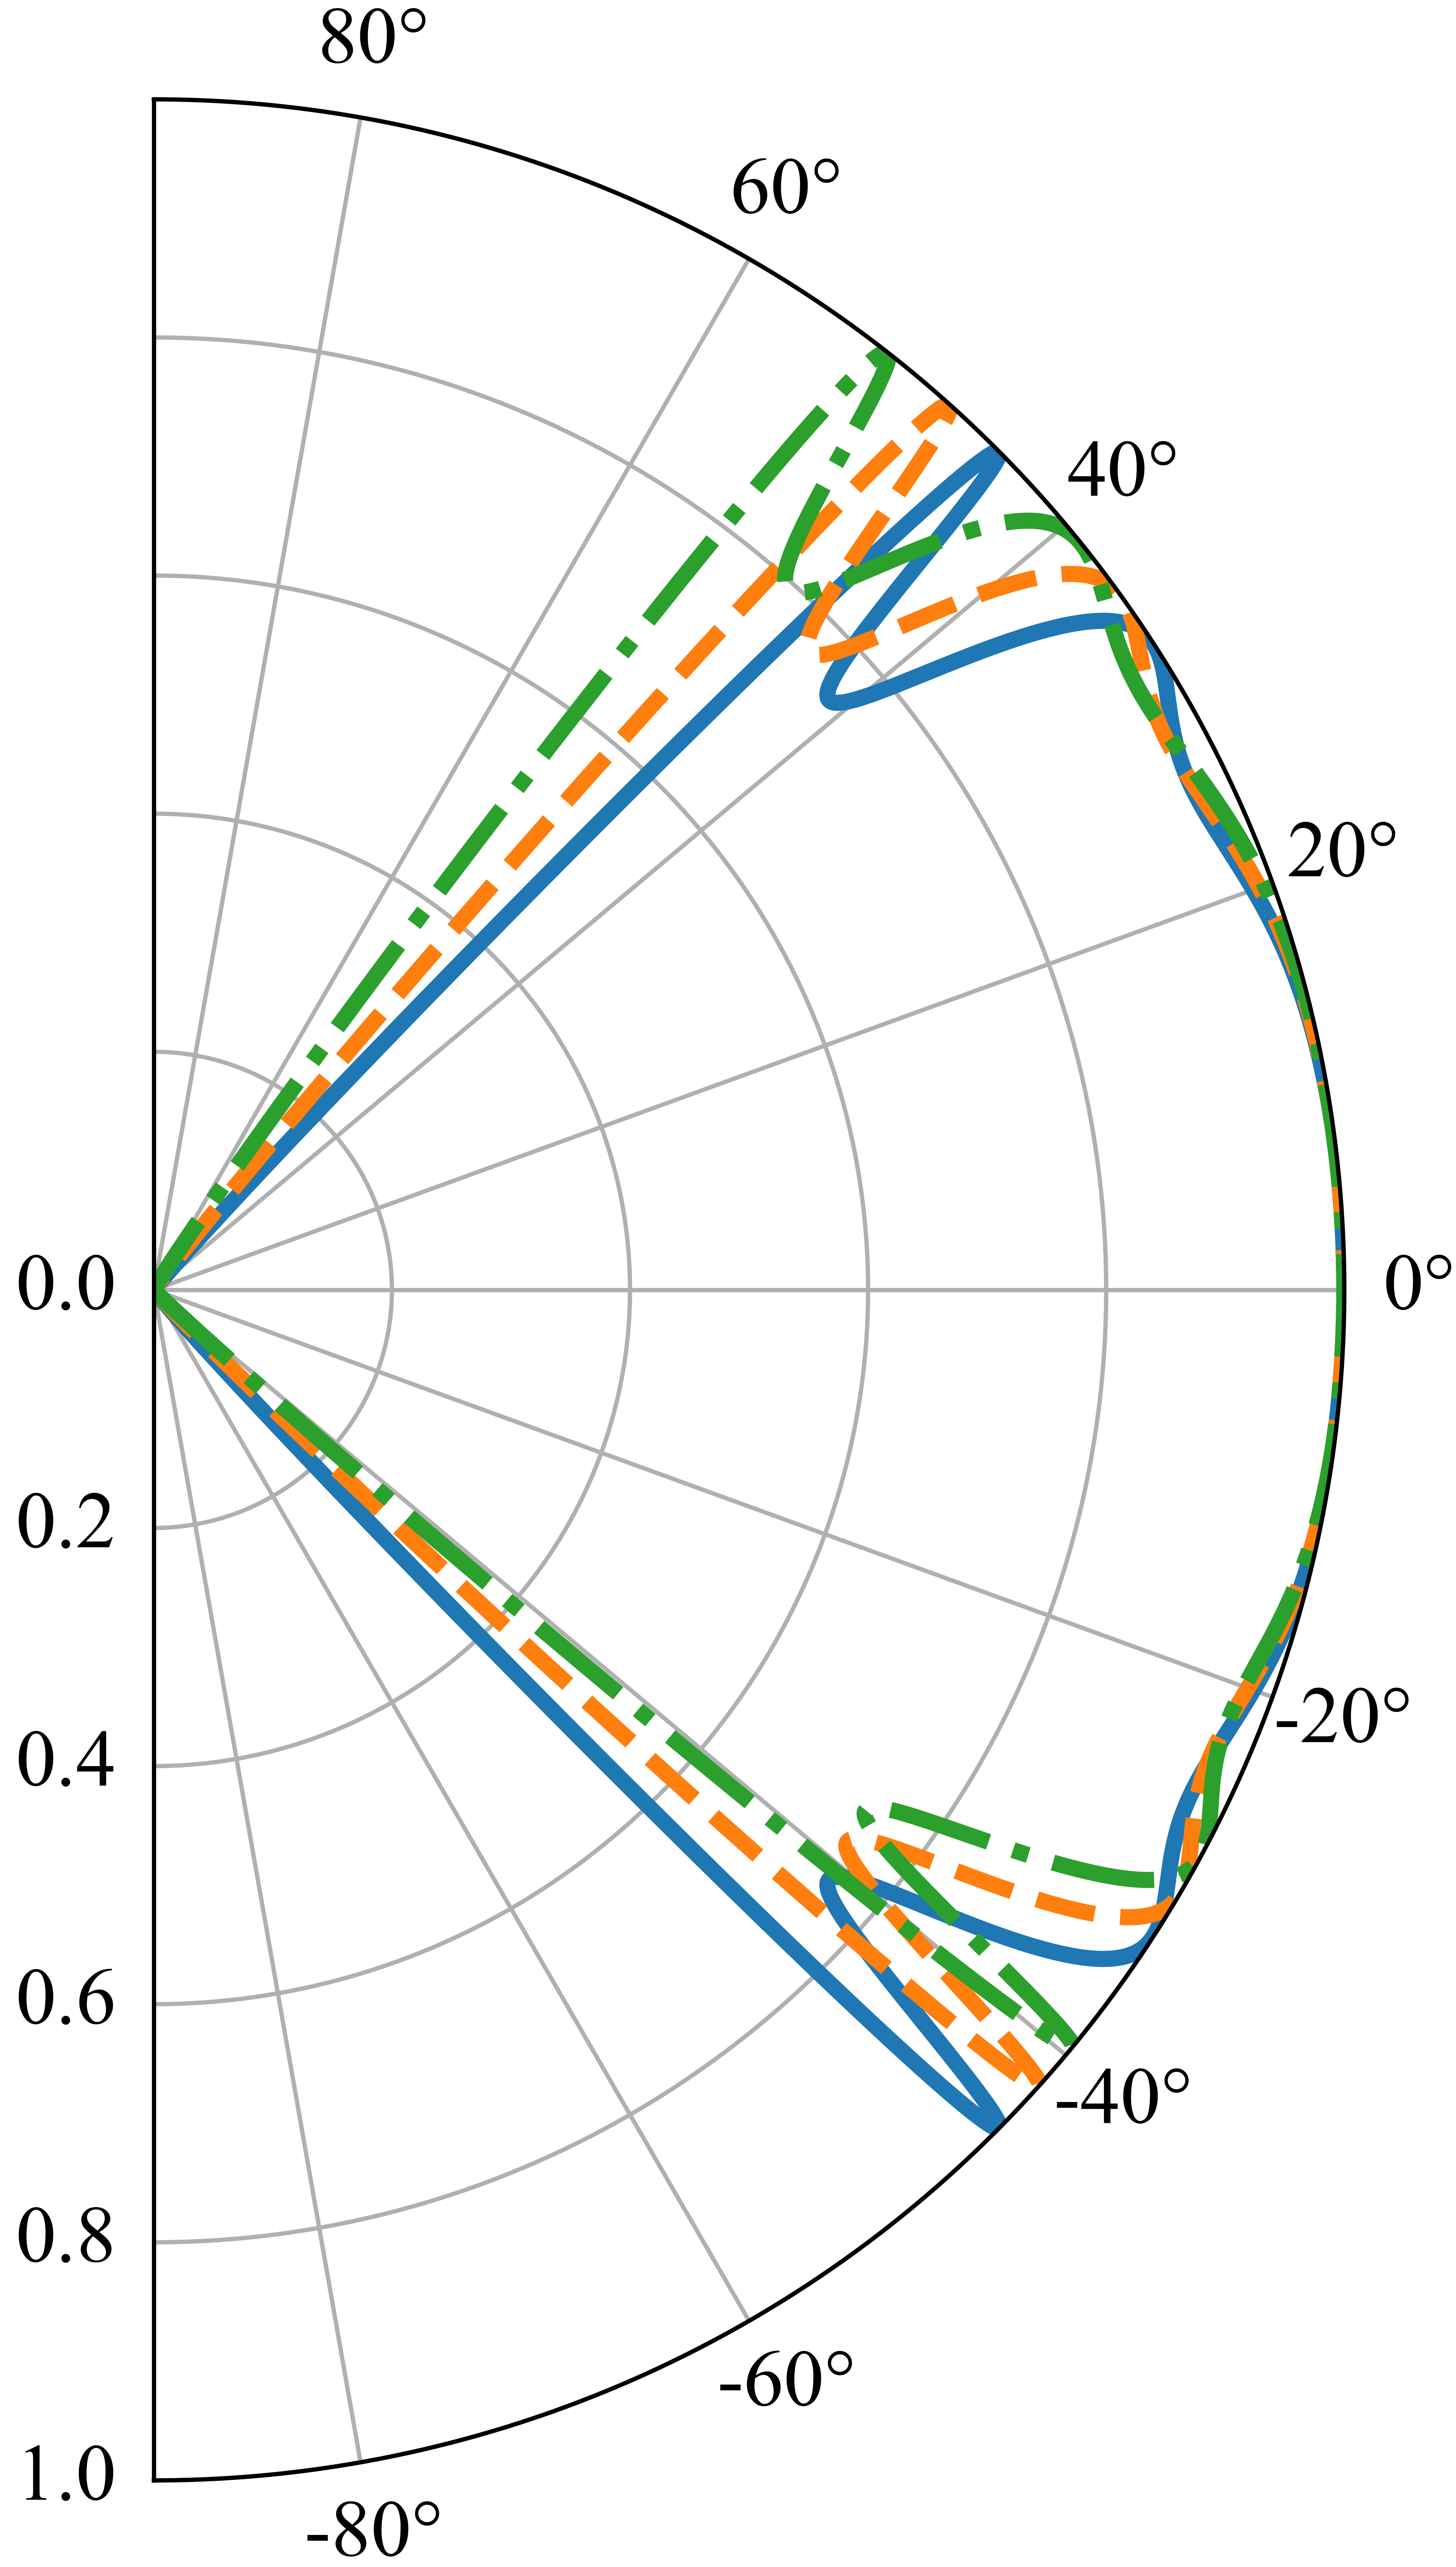
\includegraphics[width=\linewidth]{fig/tunneling shift/U0.02.png}
            \caption{}
            \label{fig:asym1}
        \end{subfigure}
        \begin{subfigure}[b]{0.3\linewidth}
            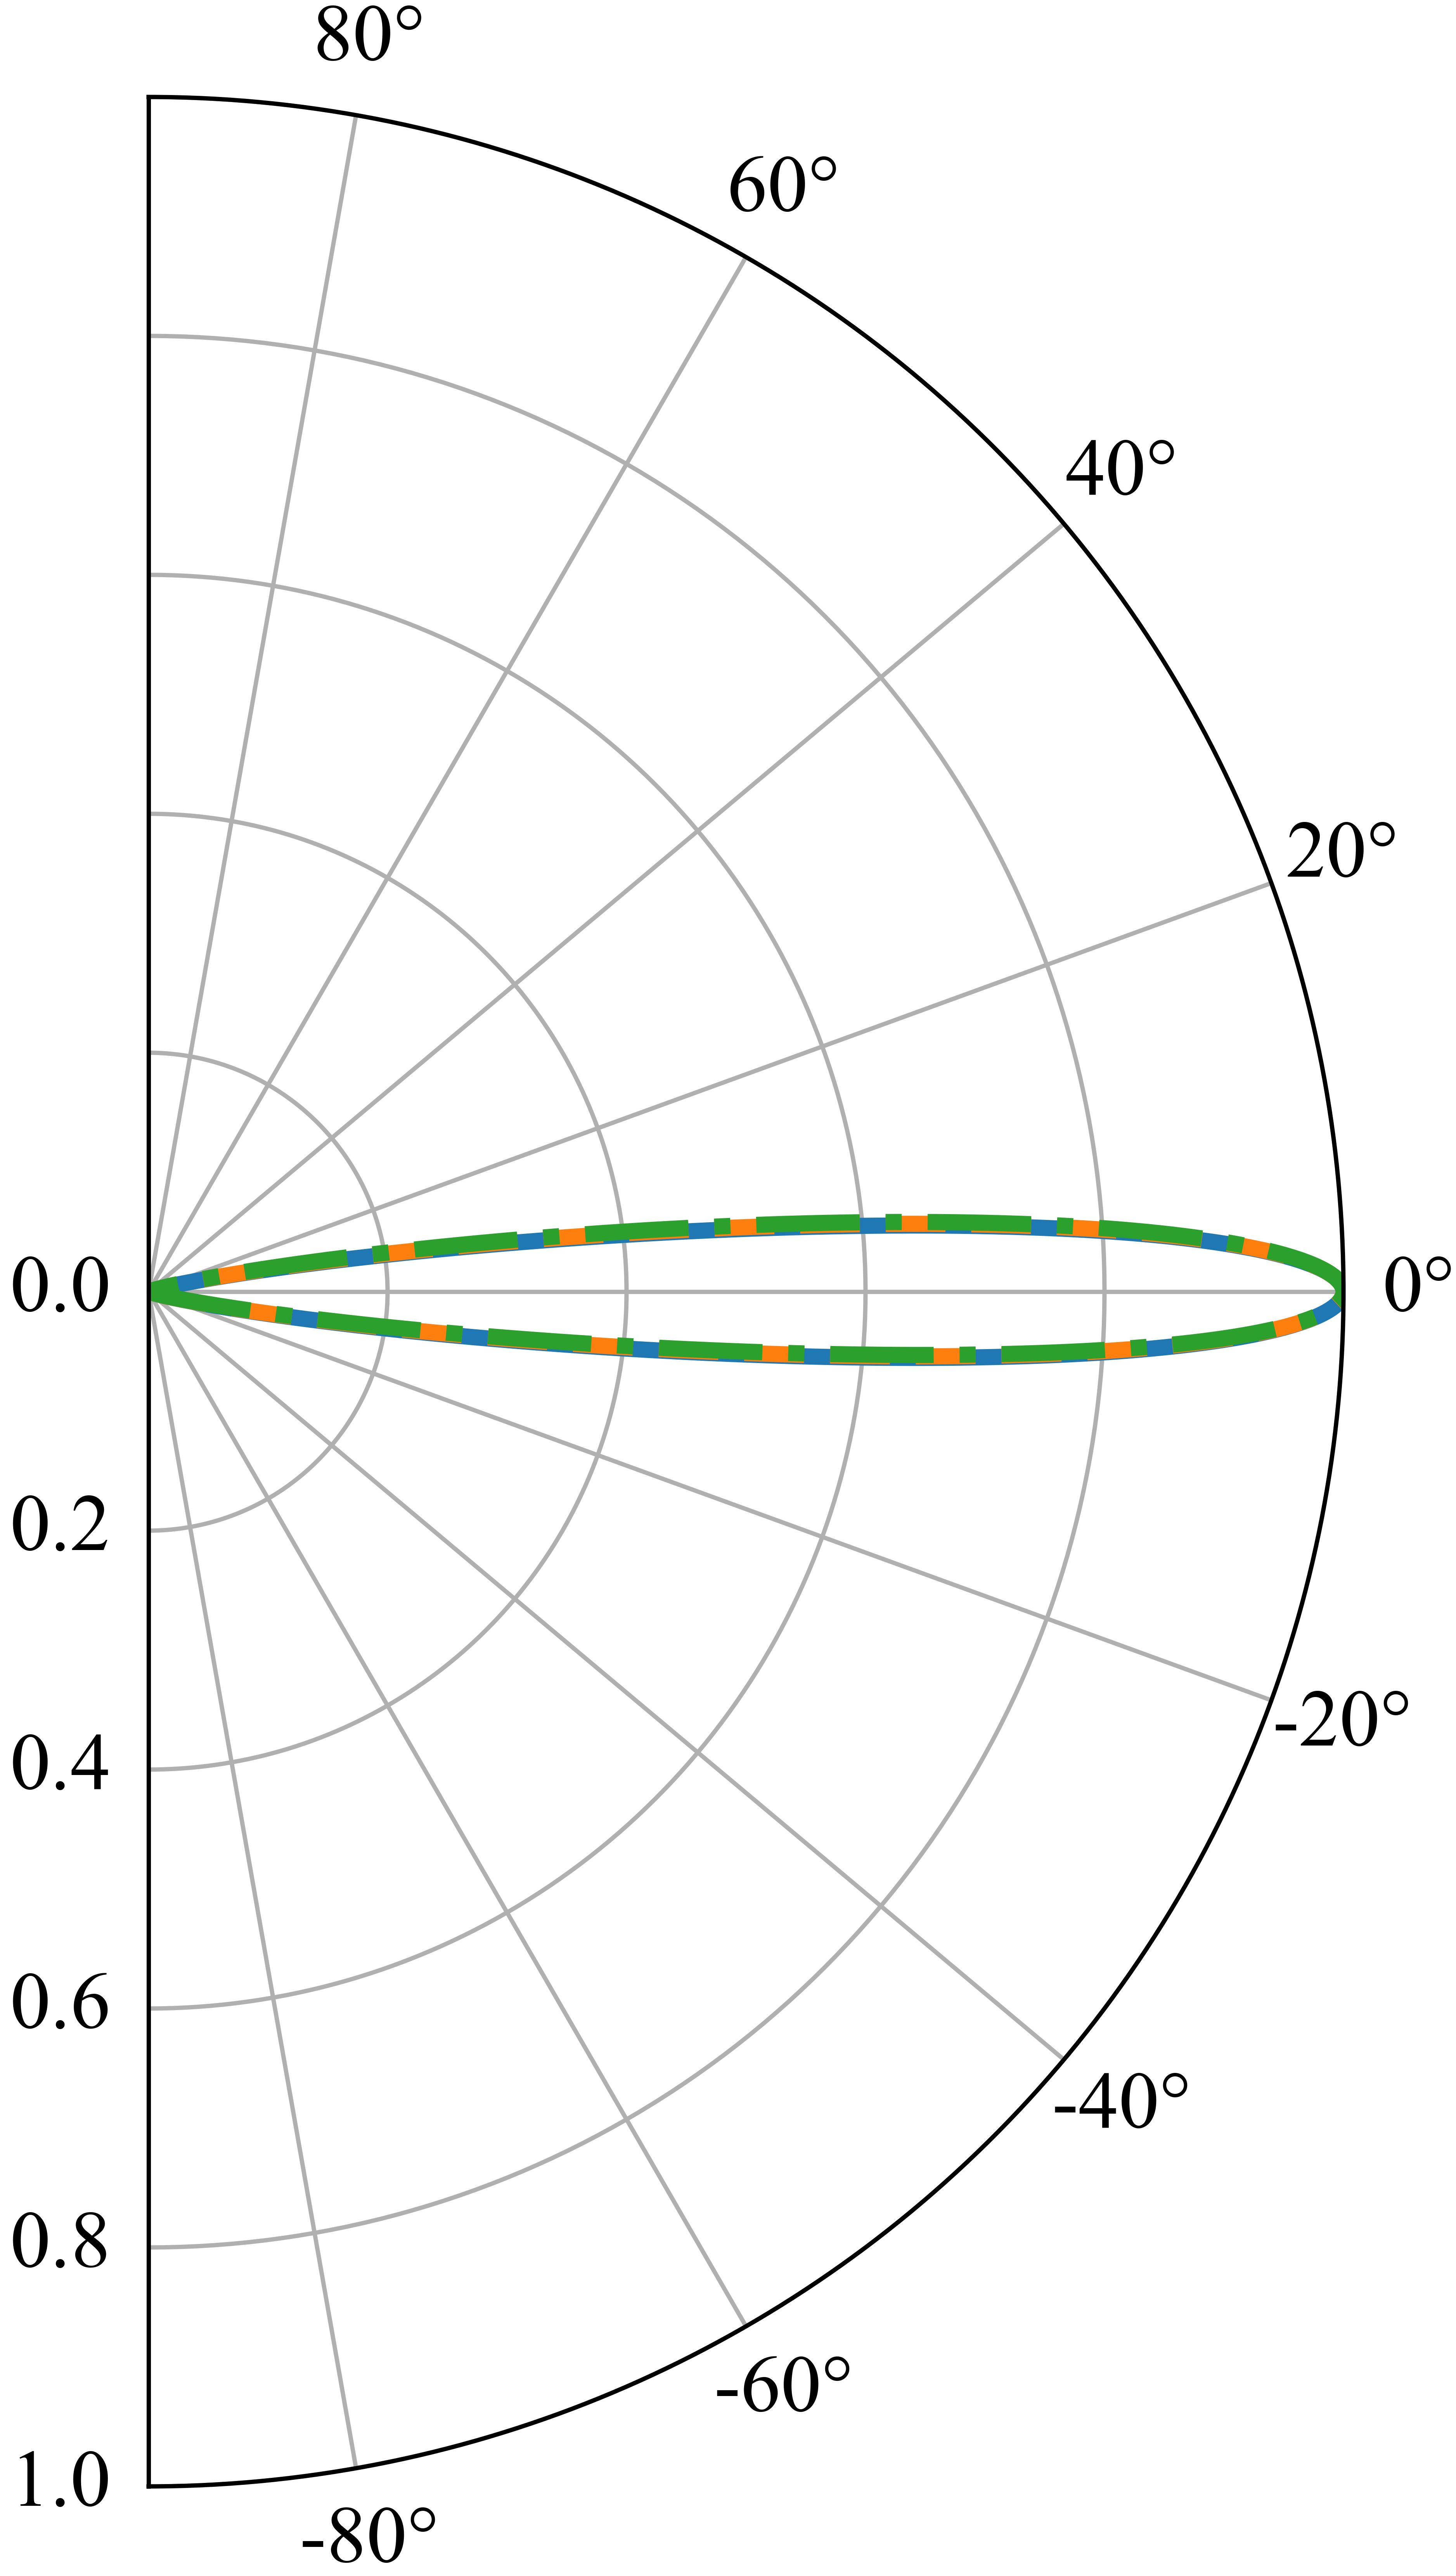
\includegraphics[width=\linewidth]{fig/tunneling shift/U0.07.png}
            \caption{}
            \label{fig:asym2}
        \end{subfigure}

        \begin{subfigure}[b]{0.3\linewidth}
            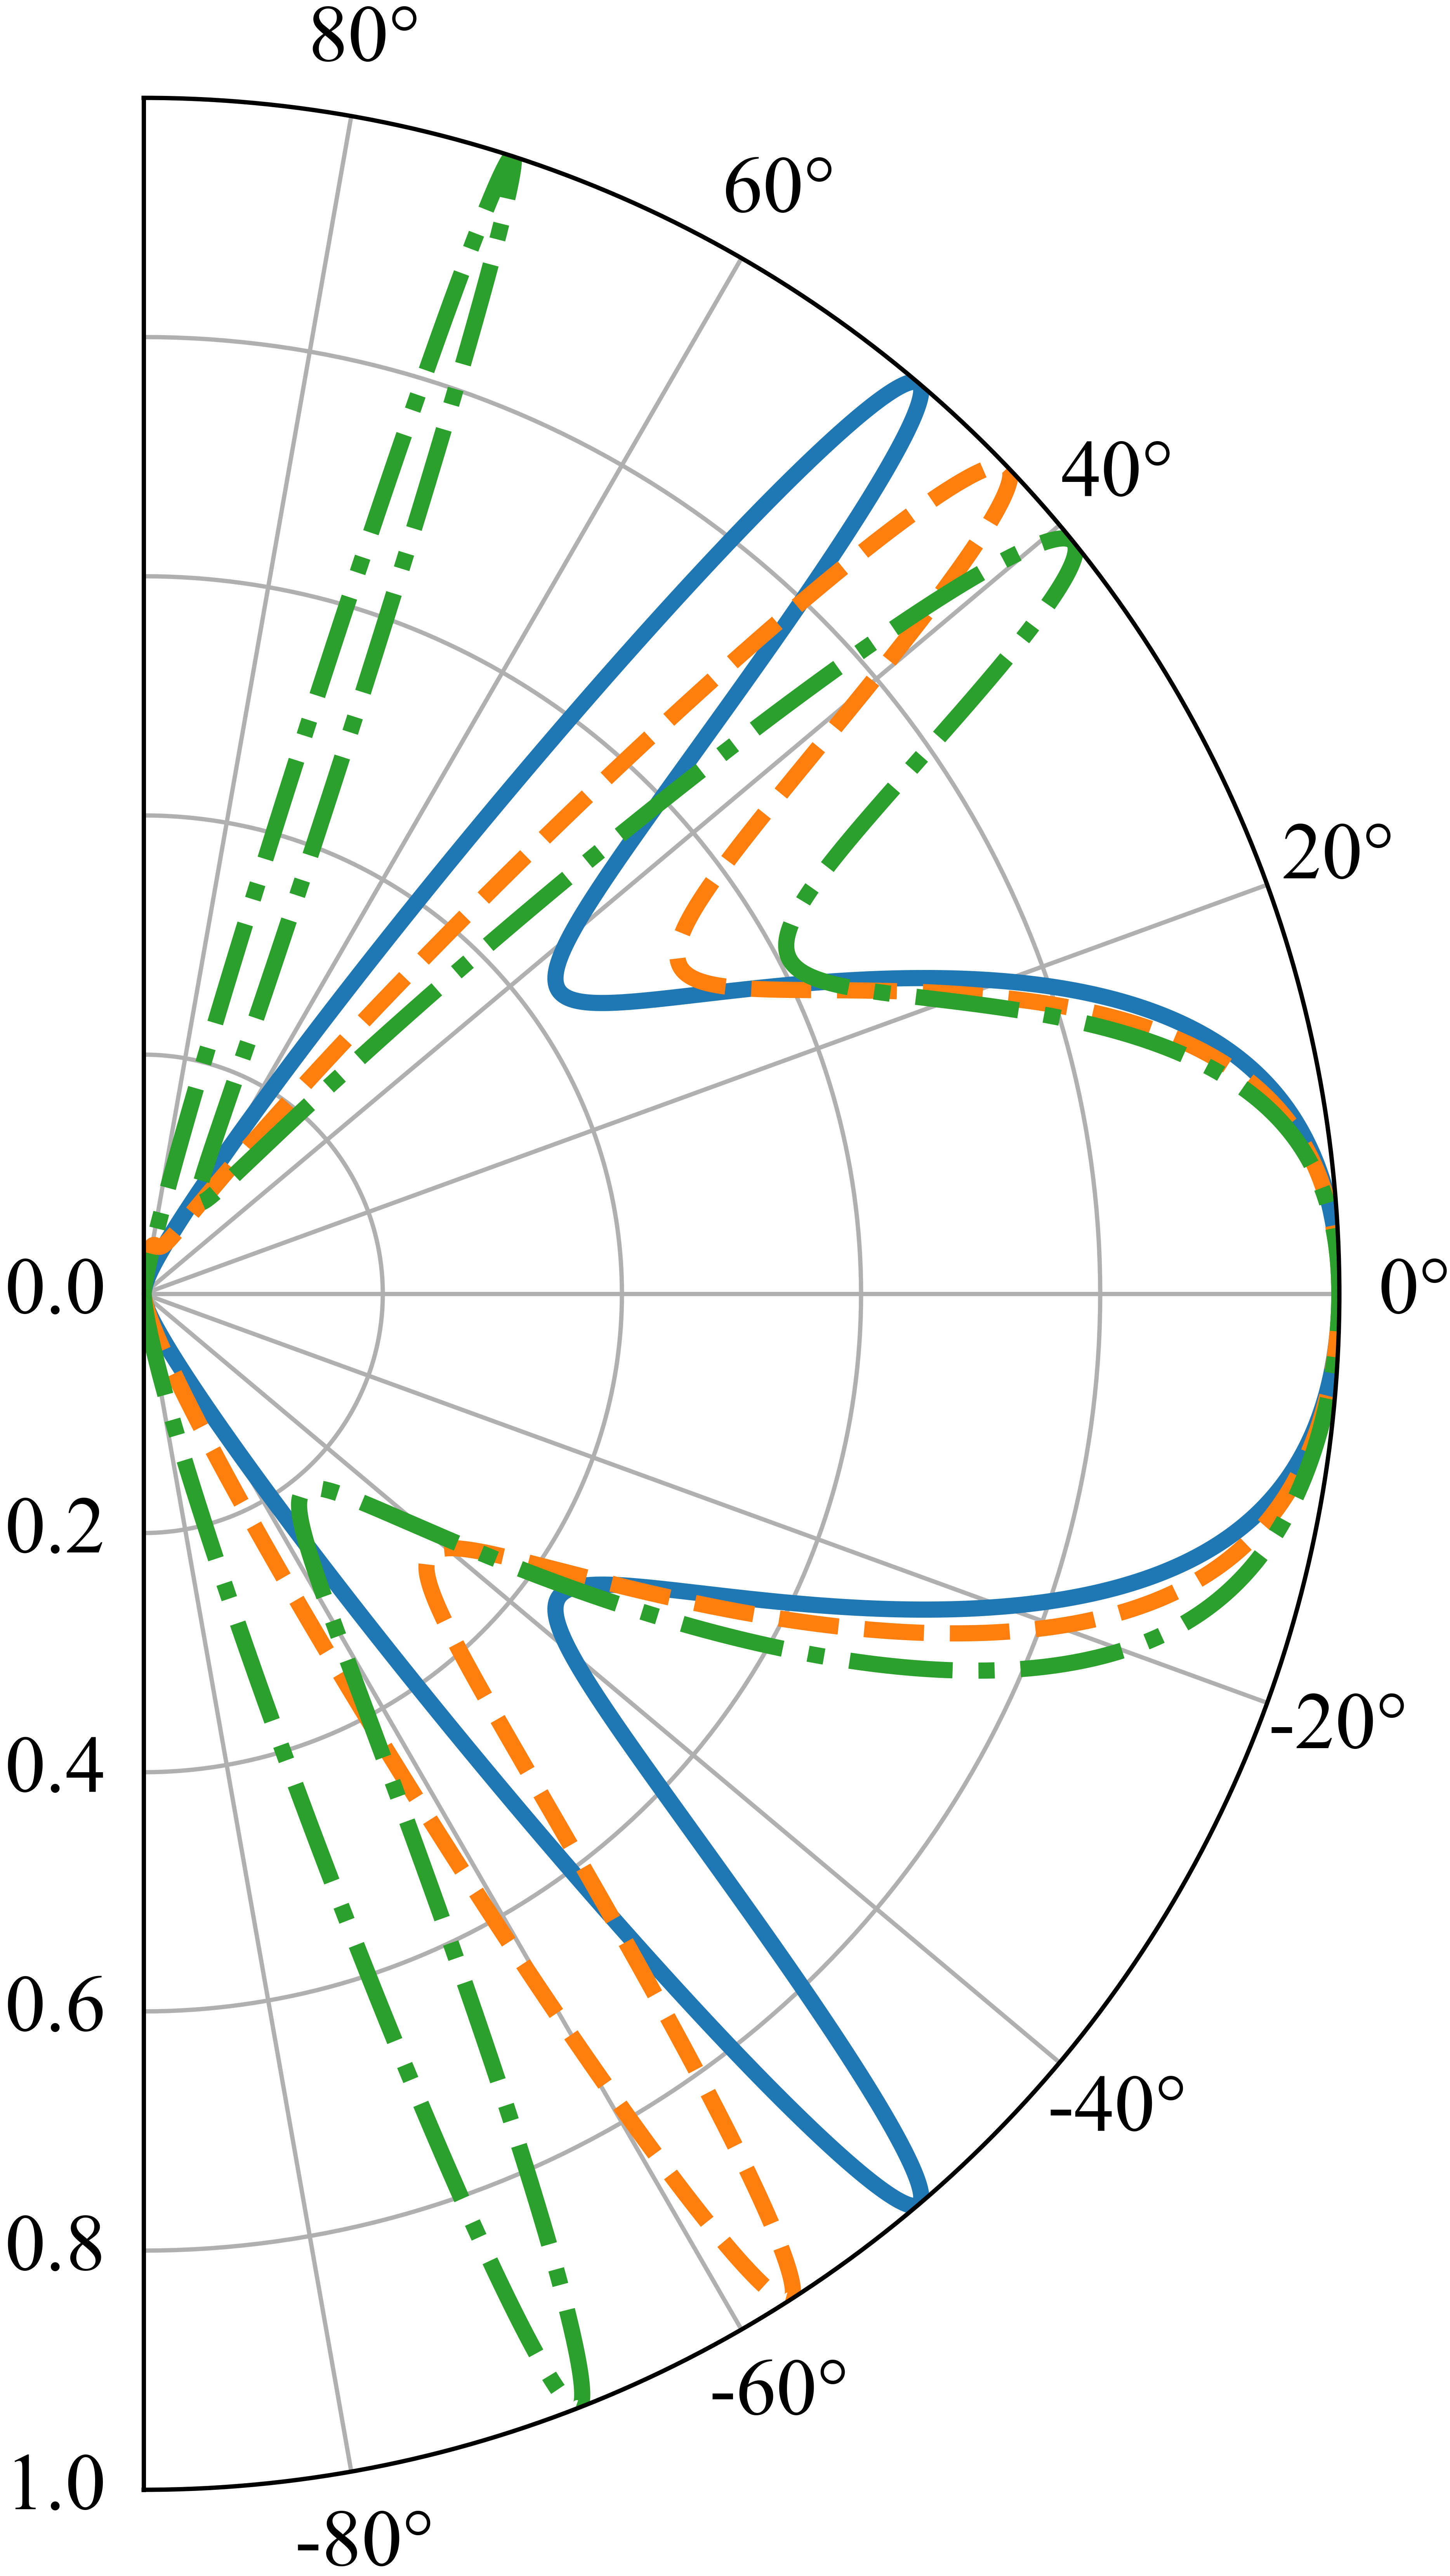
\includegraphics[width = \linewidth]{fig/tunneling shift/U0.2.png}
            \caption{}
            \label{fig:asym3}
        \end{subfigure}
        \begin{subfigure}[b]{0.3\linewidth}
            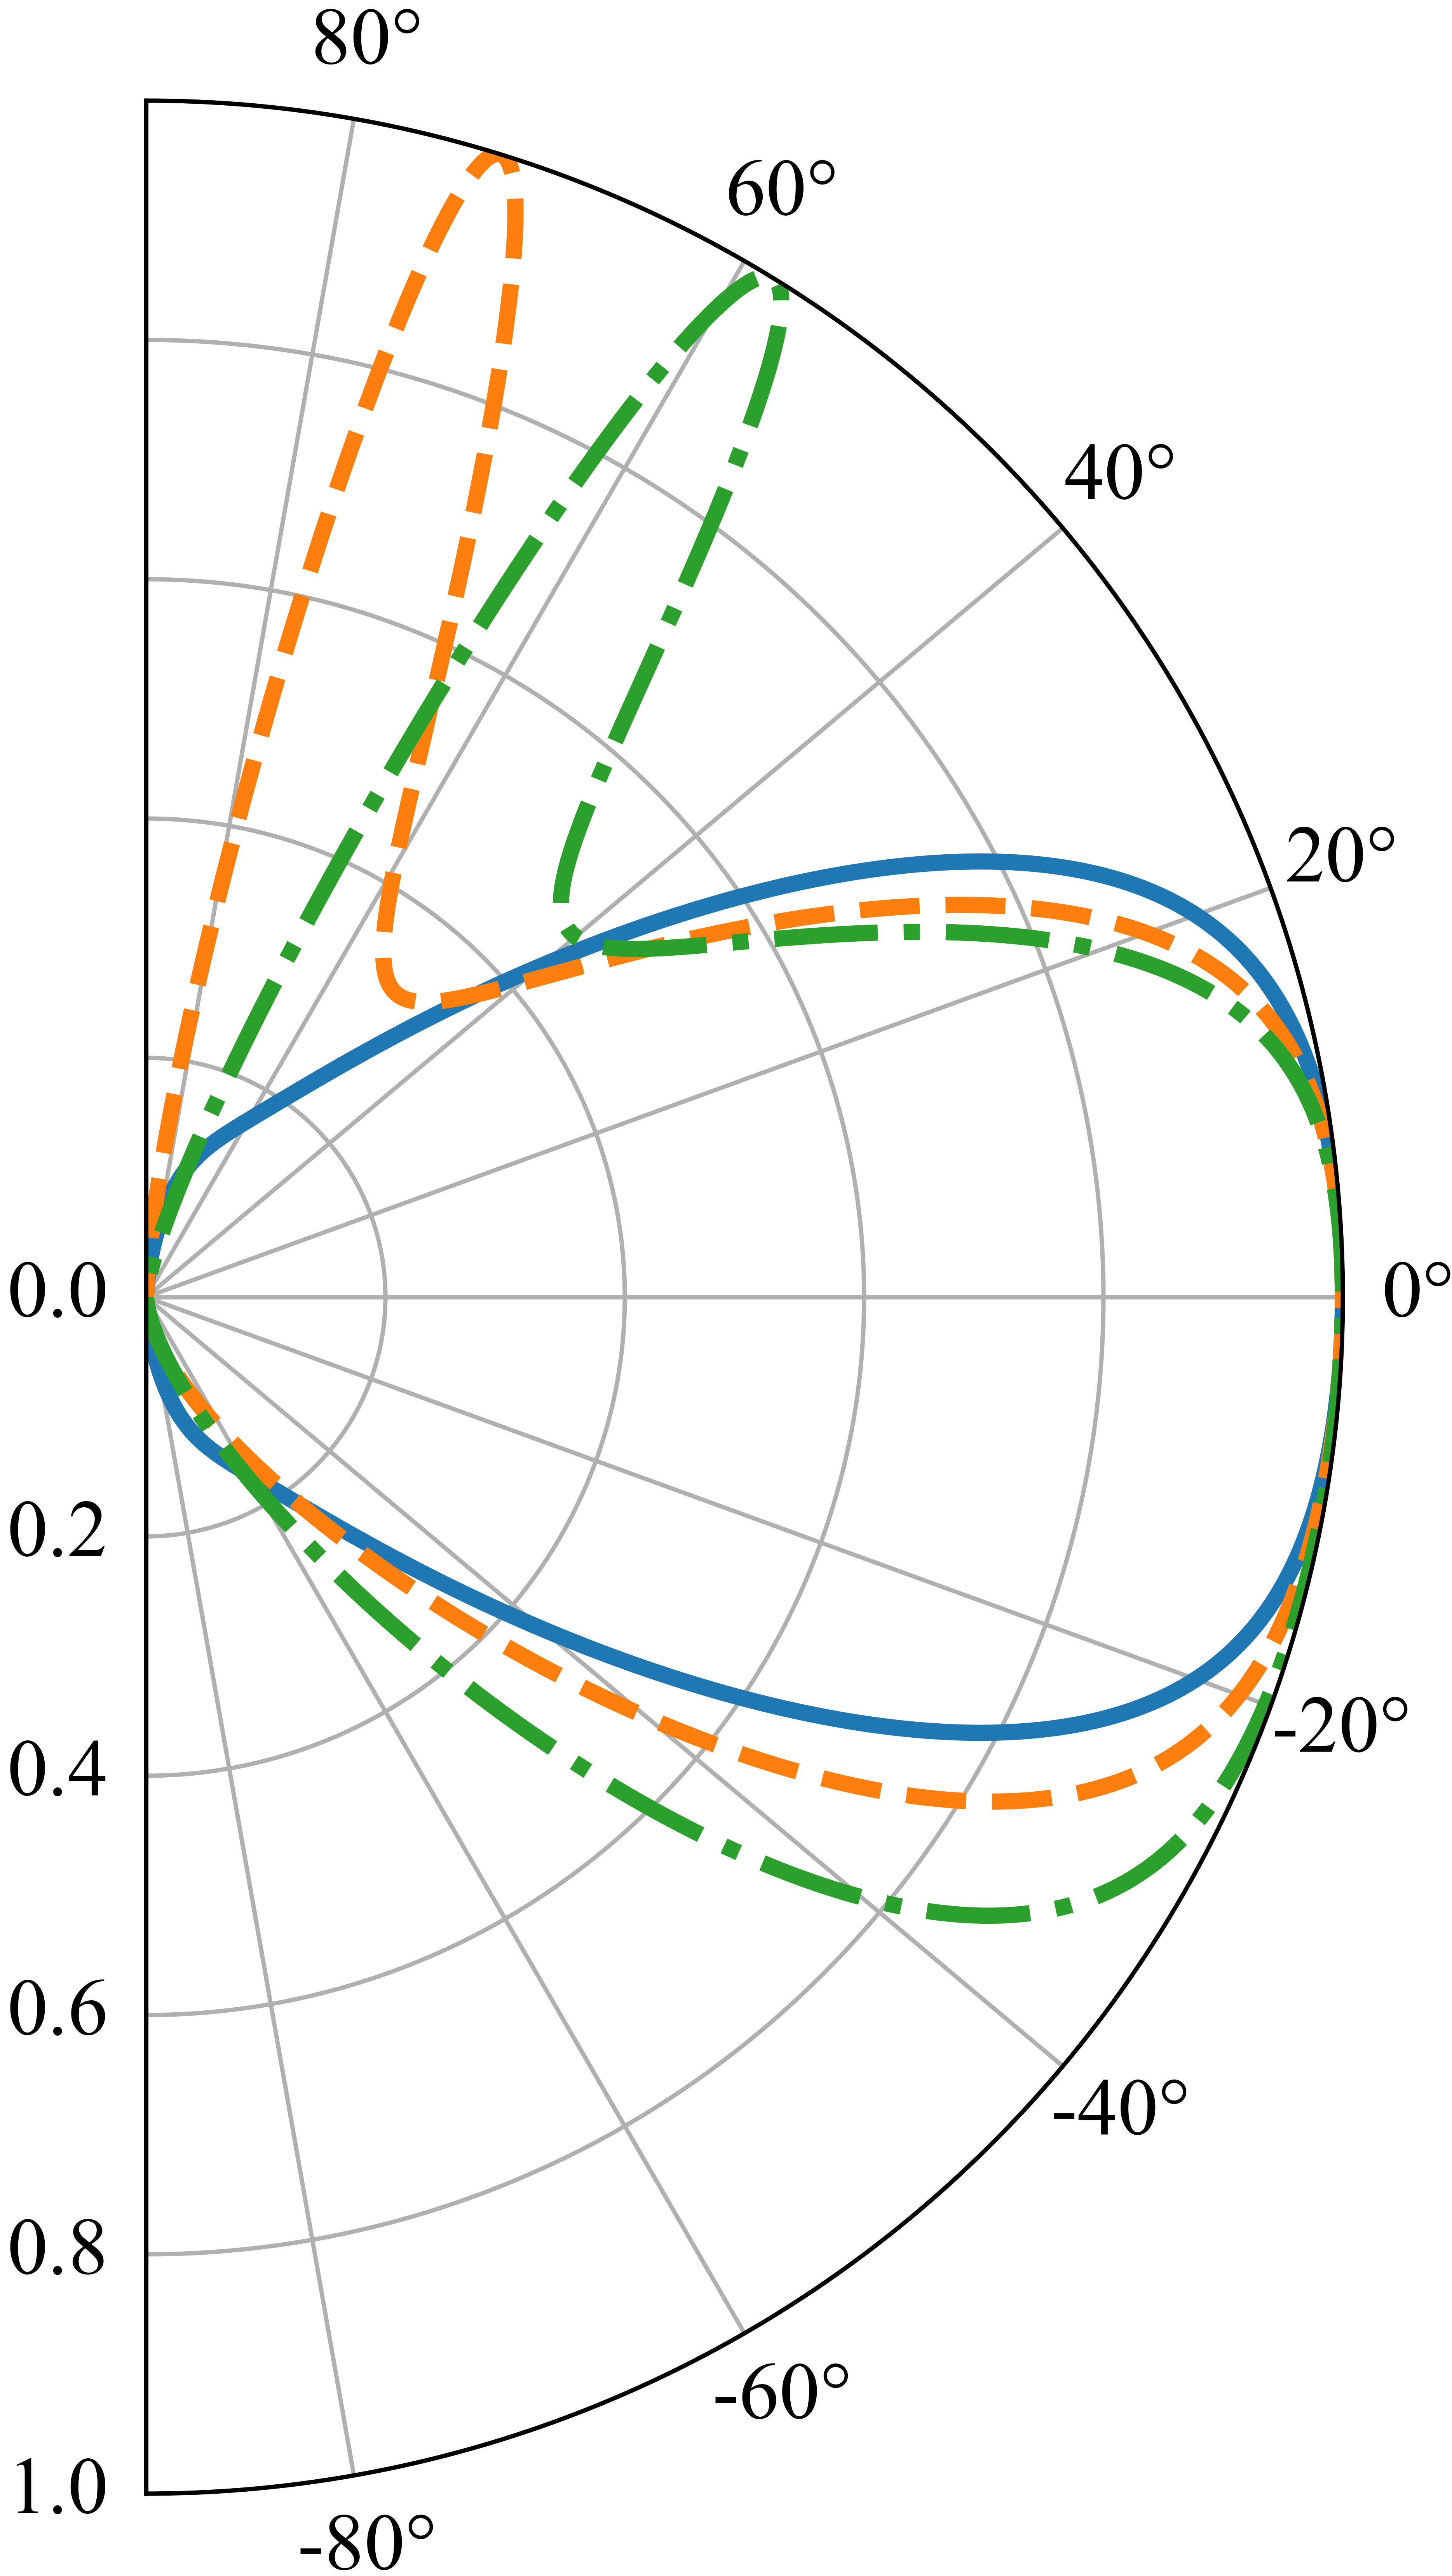
\includegraphics[width = \linewidth]{fig/tunneling shift/U0.285.png}
            \caption{}
            \label{fig:asym4}
        \end{subfigure}
        \caption{The same cup of coffee. Two times.}
        \label{fig:asym}
    \end{figure}

\section{The tilted strength identification by means of the tunneling resonance properties} \label{sec:find w}
    The resonant tunnelings are arisen if the given $U, E_F$ and, $w_0$ satisfy the resonance condition.
    Modulating these parameters result in shifting of resonant tunneling angles as previously reported in section \ref{sec:asym}.
    In this section, we demonstrate that by measuring the asymmetric resonant tunneling angles, the tilted parameter can be determined.
    Consider the resonance condition
    %by tracking how much those resonance conditions are shifted
    \begin{align} \label{eq:w0}
        L \sqrt{\left( \frac{E_F-U}{\hbar v_F}+ w_0 k_y \right)^2 -k_y^2} = n \pi \notag\\
        w_{0 \pm} = \frac{U-E_F}{\hbar v_F k \sin{\phi}}\mp \sqrt{1+\left(\frac{n \pi}{k L \sin{\phi}}\right)^2}
    \end{align}
    where subscript $+(-)$ satisfy the positive(negative) angle $\phi$ region.
    One can obtain the tilted parameter by applying the gate voltage and Fermi energy then measure the resonant tunneling angle, which can be experimentally observed
    by four-point probes technique \cite{Rahman2015}.
    To illustrate how to calculate for the tilted parameter, we substitute the configuration of dashed-dotted line in Fig. \ref{fig:asym3} to Eq. \ref{eq:w0}.
    We choose the resonance condition $n=4$, which corresponds to the resonant tunneling angle $\phi = 72^{\circ}$. We find $w_0 = 0.1$.\\
    
    However, this method is not at all practical since the variable $n$ is unlikely observable.
    Also, the only way to manipulate the electron propagations is by tuning the voltages through the bottom and top gate.
    In section \ref{sec:find w 2}, we propose a more practical method to identify the tilted strength, which again, involve with the resonant tunneling behaviors.

    %When the voltages are applied to the system, there will be 
    %For some given value of $U, E_F, \mathrm{and} $ 
    %resonance condition can be modulated by tuning $U, E_F$ and, $w_0$ since $q_x$ depends on these parameter. 
    %Electron propagations at normal incident undergo the Klein tunneling effect, where the transmission probability always equal to one.
    % the downside of this method is there are unknown parameter such as n
    %In the next section, we show how to get rid of n
\section{Oscillatory behavior of electron resonant tunneling} \label{sec:oscillation}
    To understand the behaviors of resonant tunneling under the effect of the tilt and gate potential, 
    we plot the transmission probabilities at particular incident angle $\phi = 45^{\circ}$ shown in Fig. \ref{fig:tp 45 deg}.
    We found that the resonant tunneling oscillate with the increasing of gate voltage where the voltage difference between each resonance condition is the same.
    Also The voltages required to satisfy the resonance conditions are increased with the tilted strength.
    These resonant tunnelings are shifted uniformly with the tilted parameter, which can be confirmed mathematically by taking the derivative to Eq. \ref{eq:w0} with respect to $U$
    \begin{align} \label{eq:dw wrt U}
        \frac{d w_{0\pm}}{dU} &= \frac{d}{dU} \left(\frac{U-E_F}{\hbar v_F k \sin{\phi}}\mp \sqrt{1+\left(\frac{n \pi}{k L \sin{\phi}}\right)^2}\right) \notag \\
                              &= \frac{1}{\hbar v_F k \sin{\phi}}.
    \end{align}
    Eq. \ref{eq:dw wrt U} indicates that the tilted parameter is linearly proportional to gate voltage.
    \begin{figure}[H]
        \centering
            \includegraphics[width=\linewidth]{fig/tp Ef = 0.08 e1 = 0 e2 = 0.05 e3 = 0.1.png}
            \caption{tp fixed angle}
        \label{fig:tp 45 deg}
    \end{figure}

\section{Revisit: The tilted strength identification by means of the tunneling resonance properties} \label{sec:find w 2}
    In section \ref{sec:find w}, we have demonstrated a method to identify the character of Dirac cone using the resonant tunneling properties.
    The method can be applied to any resonance condition given that we have known its corresponding resonant tunneling angle.
    However, it is still not a practical method since the parameter $n$ is unobservable.
    Also, most device configurations have fixed angled probes to observe the resonant tunneling current.
    In this section, we revisit this study again and eliminate the drawbacks mentioned above.\\
    
    We have discussed earlier in section \ref{sec:oscillation} that the relation of $w_0$ and $U$ are linear with the slope of $1/\hbar v_F k \sin{\phi}$.
    For this reason, we can identify the tilted strength by measuring the difference between two voltages satisfied the same resonance condition.
    \begin{align} \label{eq:w0 2}
        \Delta w = \frac{\Delta U}{\hbar v_F k_y}
    \end{align}
    To apply Eq. \ref{eq:w0 2} to determine the tilted parameter, the voltages satisfied the same resonance condition have to be first determined,
    which can be achieved using the device structure depicted in Fig. \ref{fig:3 arms}. We have to tune $U$ until the resonant tunneling occurs at $\phi = \pi/4$,
    where the electron current can be measured as shown in Fig. \ref{fig:tp at 45 deg}.
    The voltage at which the resonant tunneling occurs at $\phi = \pi/4$ for the case of non-tilted Dirac cone can be easily obtained since it is the system found in pristine graphene.
    Substituting these gate voltages to Eq. \ref{eq:w0 2} we obtain $w_0 =0.1$
    %we can have 
    %we apply the linear relation of $w_0$ and $U$, that we discussed in section \ref{sec:oscillation}, 
    %We can pick any of these resonance condition and find its corresponding gate voltage
    %the tilted parameter can be identified by calculating the voltage difference of that resonance condition 

    \begin{figure}[H] 
        \centering
        \begin{subfigure}[b]{0.45\linewidth}
            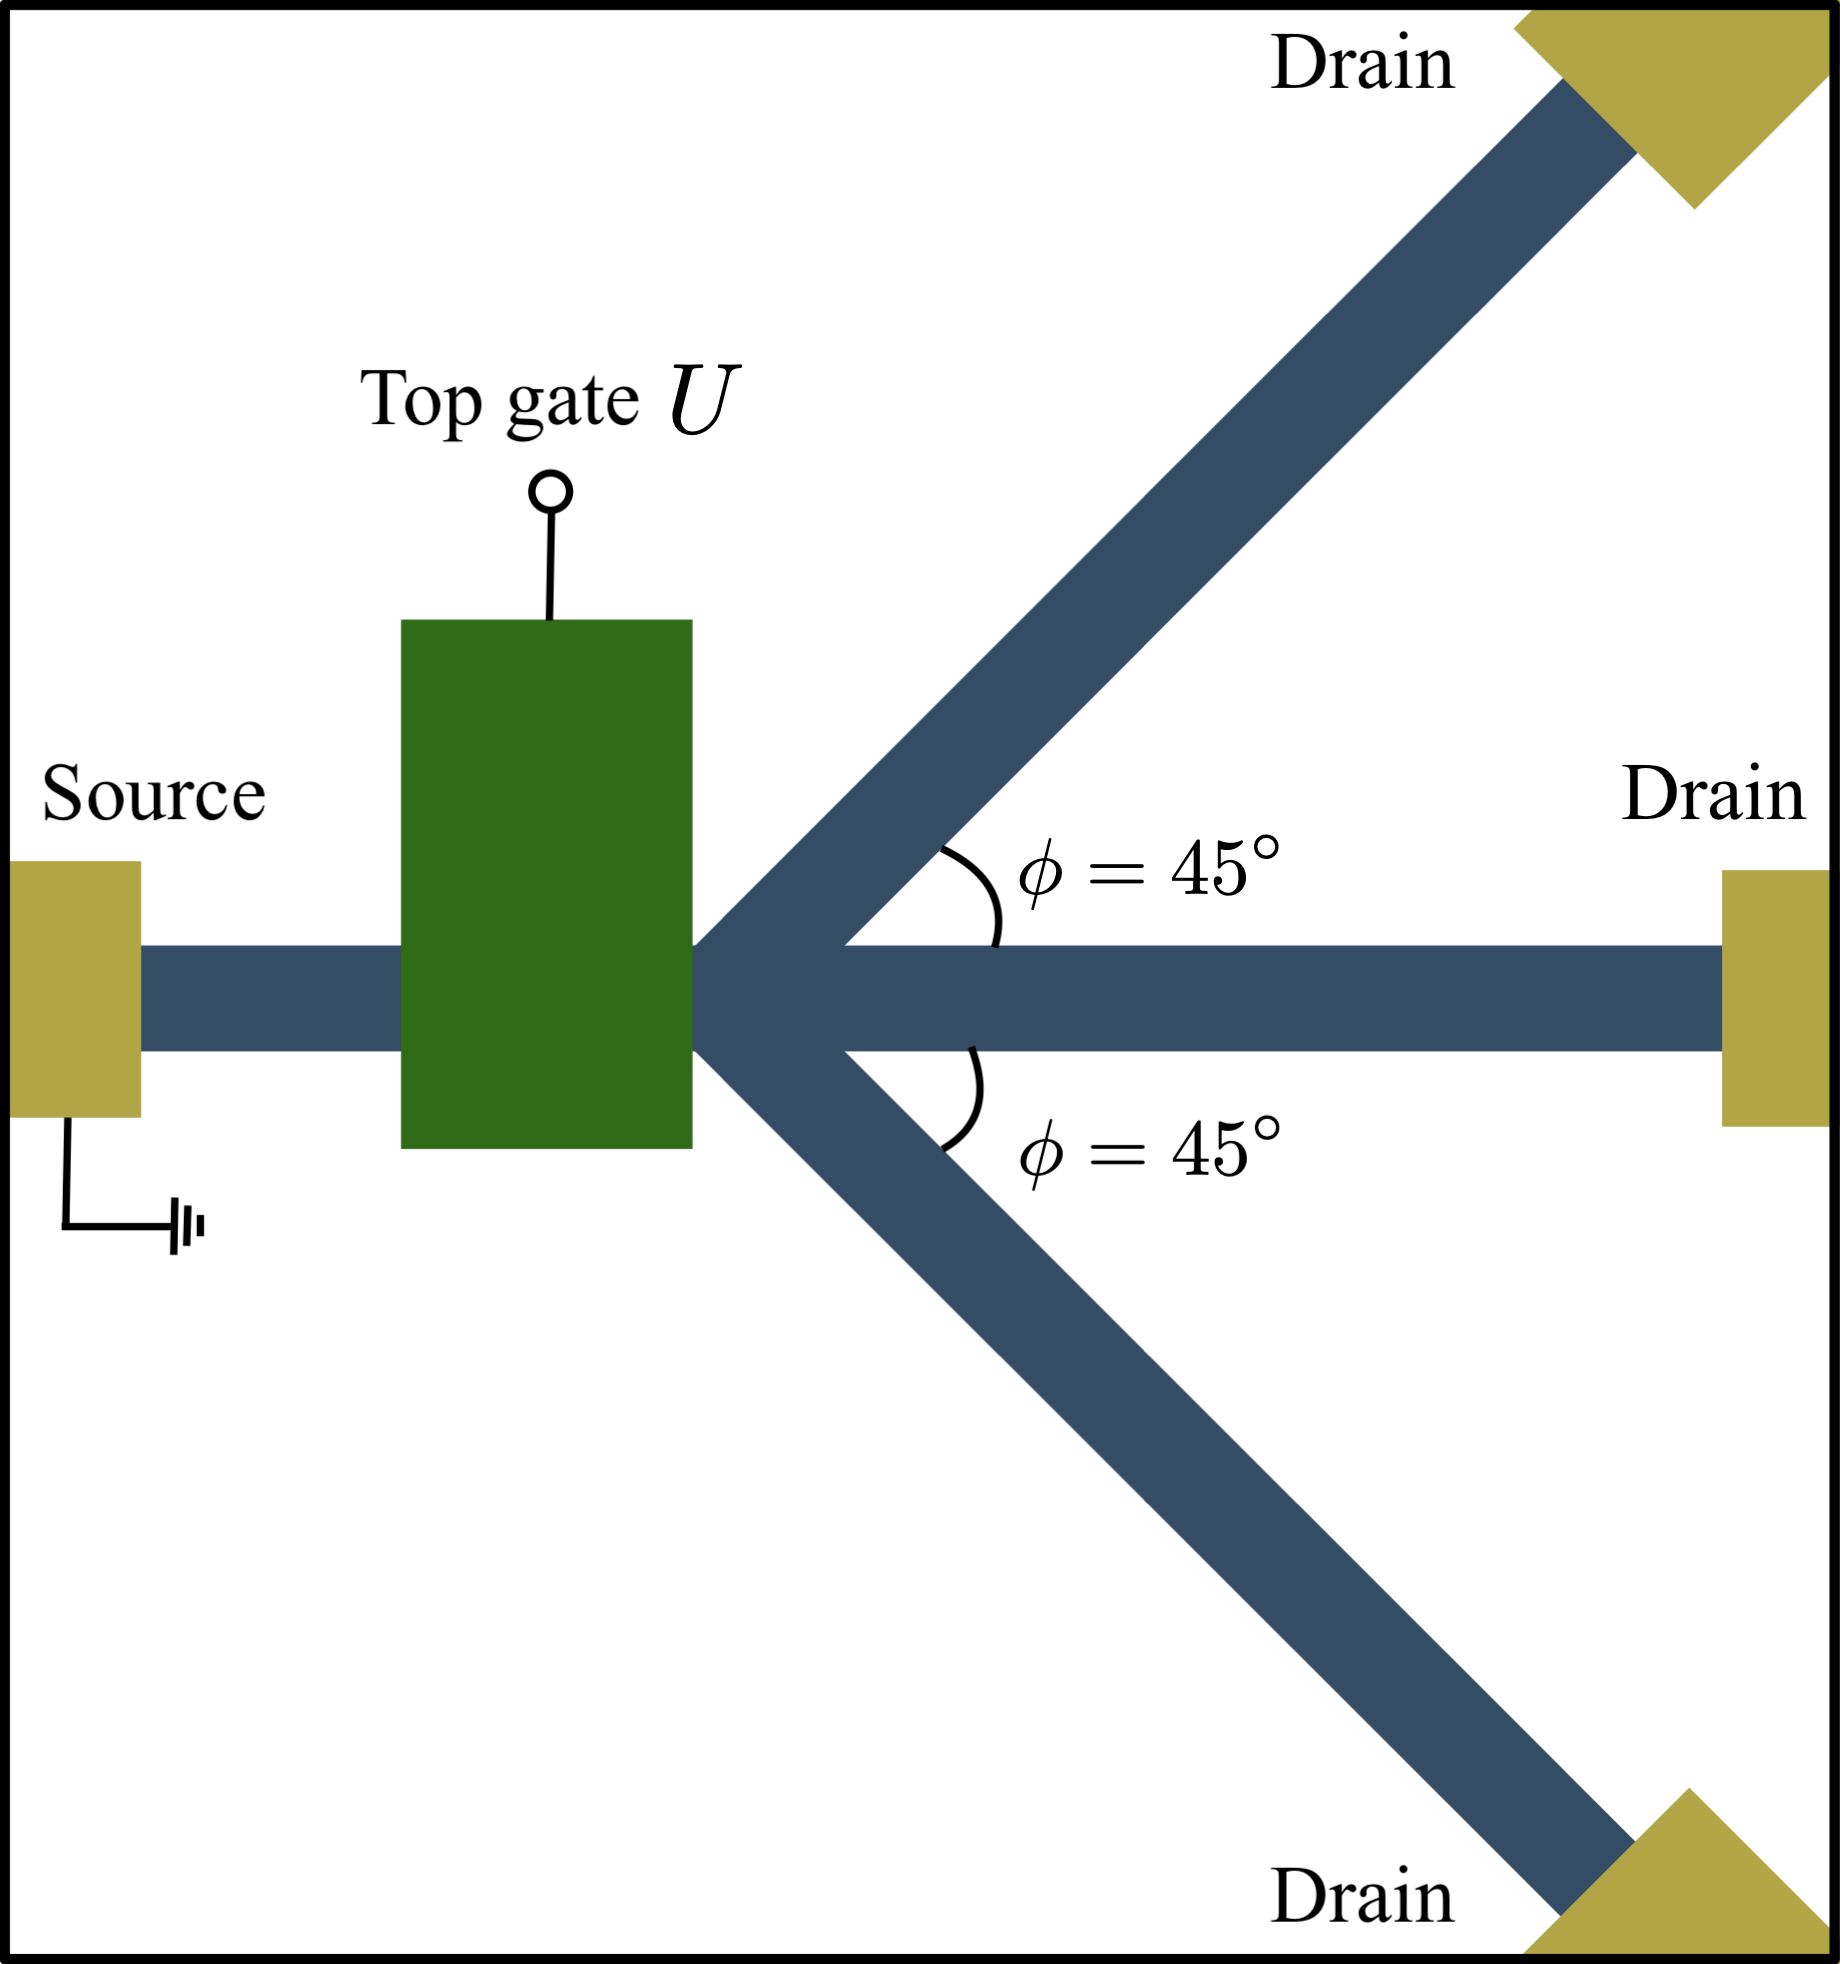
\includegraphics[width=\linewidth]{fig/3 arm structure.png}
            \caption{}
            \label{fig:3 arms}
        \end{subfigure}
        \begin{subfigure}[b]{0.3\linewidth}
            \includegraphics[width=\linewidth]{fig/tp Ef = 0.08 U1 = 0.1802 e1 = 0 e3 = 0.1.png}
            \caption{}
            \label{fig:tp at 45 deg}
        \end{subfigure}
        \caption{(a) The device structure for the measurement of resonant tunneling electron.  
                    Straight blue lines represent the transport region where both arms are $45^{\circ}$ angled with the normal direction. 
                    Green and yellow region represents top gate and electrode respectively. 
                    (b) Angular-dependent transmission for different applied voltages, U=180.2 meV for solid line and U=185.85 meV for dashed-dotted line. 
                    These voltages satisfy the resonance condition at $\phi = \frac{\pi}{4}$.}
        \label{fig:find w}
    \end{figure}
\section{Pseudo magnetic field} \label{sec:pseudo b}
    In section \ref{sec:asym}, we have shown that the tunneling behavior of electron across the tilted Dirac cone exhibits asymmetric transmission. 
    Previously, the transmission of this kind can be achieved by applying the magnetic barrier to the system \cite{RamezaniMasir2008,RamezaniMasir2010}.
    In this section, we demonstrate that the similar transmission profile can also be achieved in the tilted Dirac cone system without the magnetic barrier.
    Consider the x-component wavevector inside the barrier region $q_x = \sqrt{q^2-k_y^2}$, which can be rearranged into the form
    \begin{equation} \label{eq:k_shift}
        q_x \approx \sqrt{q'^2 -(k_y-q'w_0)^2}
    \end{equation} 
    where $q' = \frac{E_F-U}{\eta \hbar v_F}$. 
    Notice that the y-component wavevector in Eq. \ref{eq:k_shift} is shifted by the tilted Dirac cone similar to the wavevector shift by the effect of magnetic vector potential.
    Based on this analogy, we can derive the equivalent pseudo magnetic field
    \begin{align} \label{eq:pseudo B}
        -q' w_0 &= \frac{\xi}{l_B} \notag \\
        -\left(\frac{E_F-U}{\eta \hbar v_F}\right) w_0 &= \xi\sqrt{\frac{|e| B}{\hbar}} \notag \\
        B &= \left(\frac{\varepsilon w_0}{v_F}\right)^2 \frac{1}{\xi \gamma \hbar |e|}
    \end{align}
    where $\varepsilon = E_F-U$ is effective Fermi energy. 
    $\xi = \pm 1$ is in fact the direction of magnetic field, but since these fields are induced by the tilted Dirac cone, it can be considered as the direction of the tilt.
    The positive(negative) sign mean that the Dirac cone tilted to the left(right) side with respect to normal direction. 
    $\gamma = \pm 1$ indicate the carrier type in Fermi energy level.

\section{The key consequence of the mismatch effect}
    We have found in section \ref{sec:pseudo b} that both the potential and tilt are the source of pseudo-magnetic field effect, where the strength and direction of the field can be controlled by tuning the effective Fermi energy.
    This effect actually been proposed in Weyl semimetal n-p-n junction with tilted Weyl cones \cite{Yesilyurt2017a}.
    However, the coupling of the tilt and top gate potential barrier is required to preserve the effect. In contrast to our work, where the top gate potential can be set to zero, and pseudo-magnetic field effect still occurred according to Eq. \ref{eq:pseudo B}.
    Which is the consequence of the existence of the mismatch between Dirac cones with different tilted parameters. 
    To show how the mismatch plays an important role in mimicking the pseudo-magnetic field effect without the requirement of potential barrier. 
    We sketch the Fermi surface of the first and second regions, as shown in Fig. \ref{fig:fermi surface}, where top gate potential is set to zero. 
    Hence, electrons in both regions occupy in the same Fermi energy level. 
    If the Dirac cones are tilted homogeneously, the Fermi surface of both regions are completely overlapped. 
    Consequently, the electron can symmetrically propagate in all directions as shown in Fig. \ref{fig:real vs pseudo}. 
    When the inhomogeneity is introduced, where only the Dirac cone in the second region is tilted while the first region is vertical non-tilted. 
    The Fermi surfaces are partially overlapping as indicated by shaded area, which lead to asymmetric tunneling.
    
    \begin{figure}[H] 
        \centering
            \begin{subfigure}[b]{0.3\linewidth}
                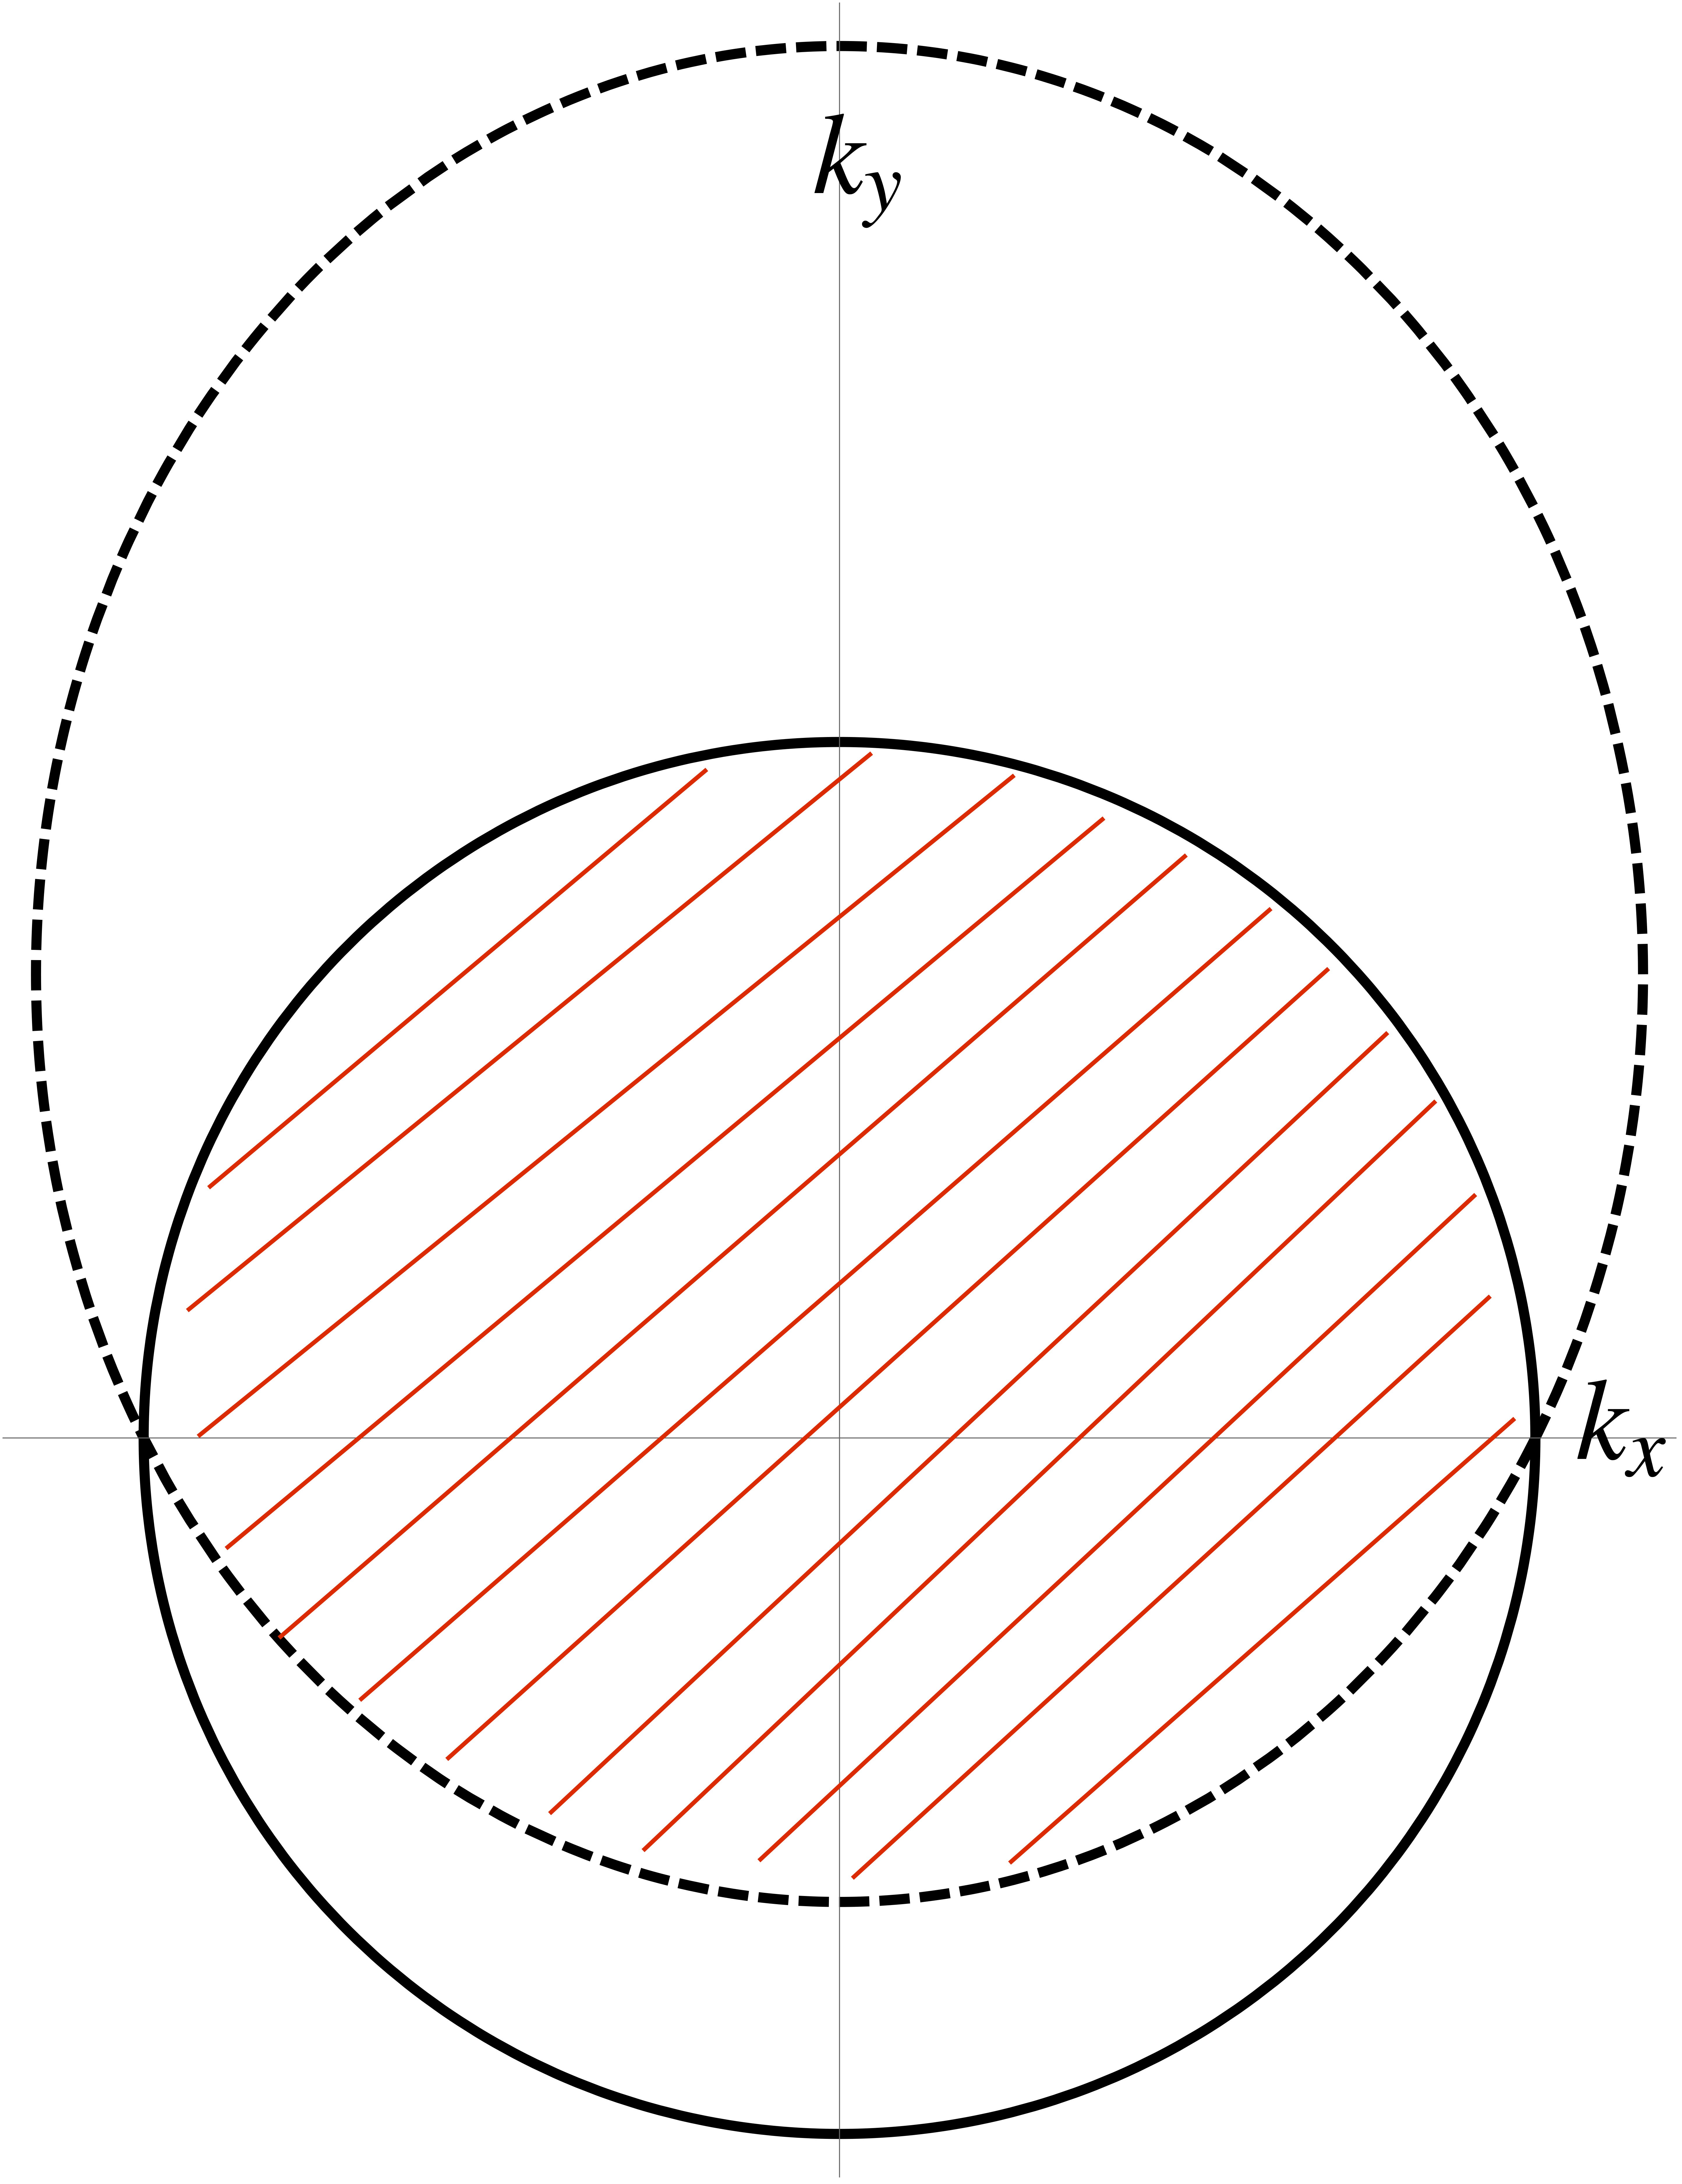
\includegraphics[width=\linewidth]{fig/Fermi surface.png}
                \caption{}
                \label{fig:fermi surface}
            \end{subfigure}
            \begin{subfigure}[b]{0.3\linewidth}
                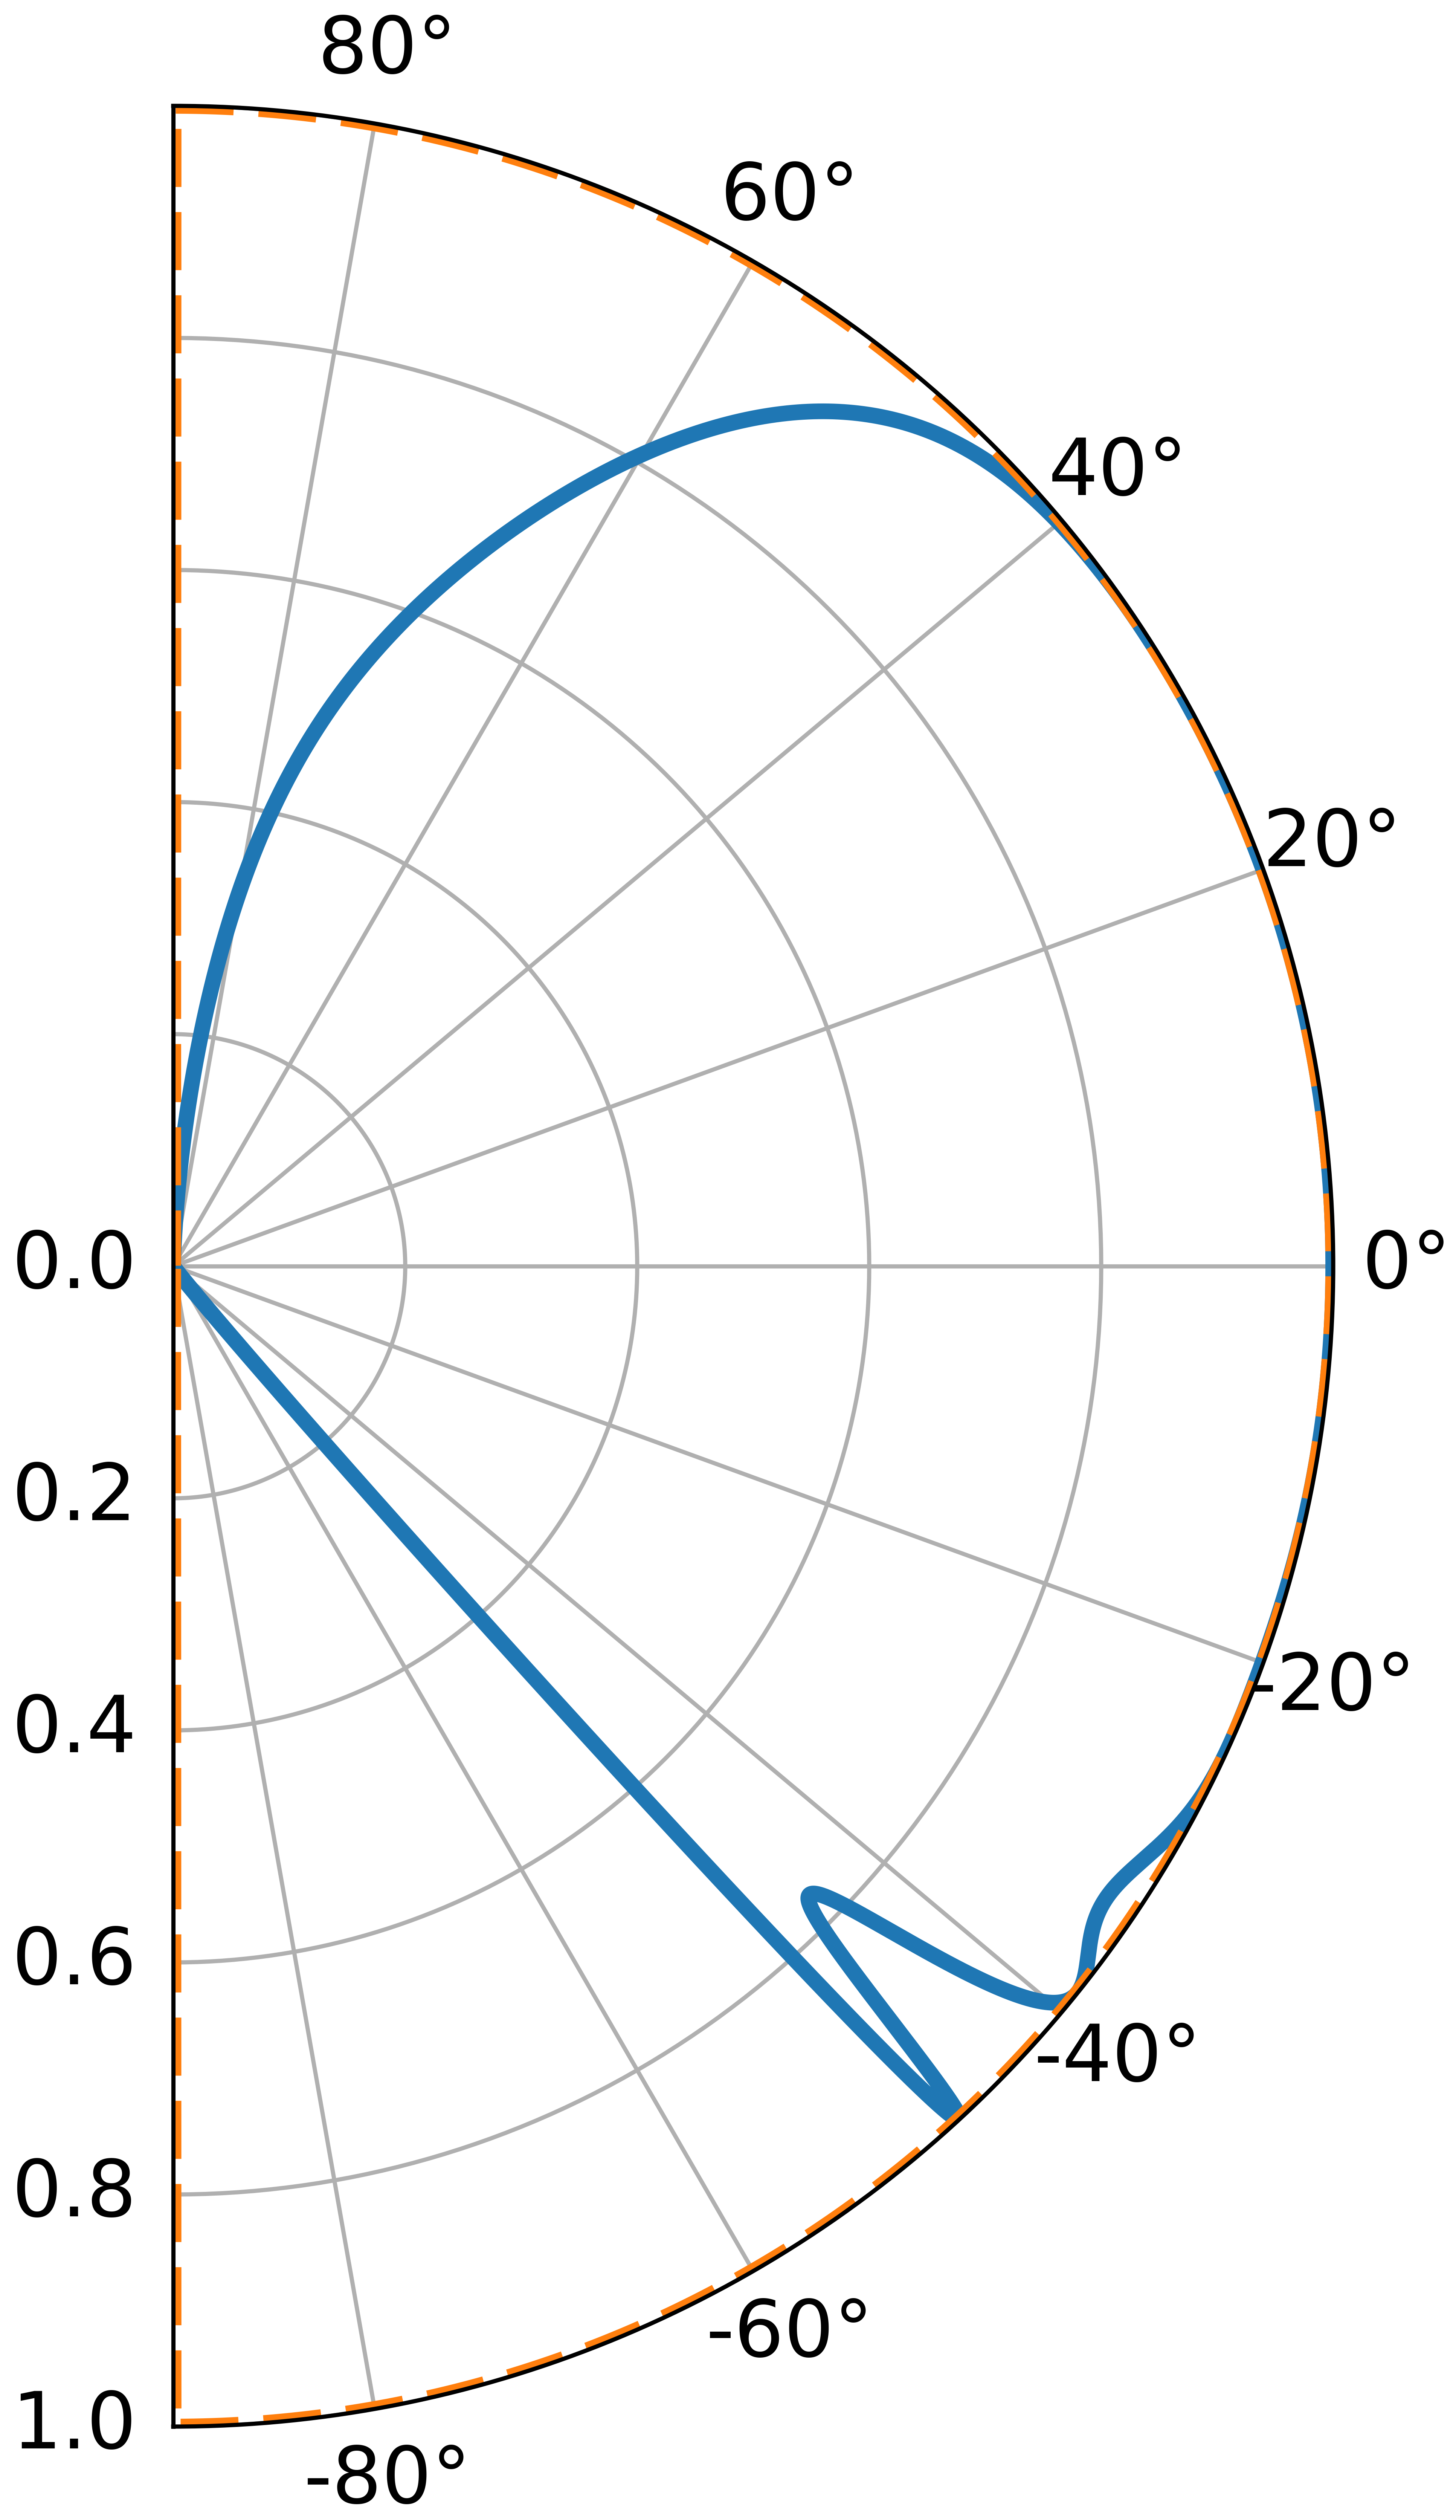
\includegraphics[width=\linewidth]{fig/real vs pseudo.png}
                \caption{}
                \label{fig:real vs pseudo}
            \end{subfigure}
        \caption{(a) The Fermi surfaces of Dirac cones in different regions. 
                    The solid line represents the Fermi surface of non-tilted Dirac cone in region I and the dashed line represents the Fermi surface of tilted Dirac cone $w_0=0.5$ in region II. 
                    (b) The transmission probabilities as a function of incident angle, where the solid (dashed) line is the case of the system with (without) the mismatch of Dirac cones. 
                    The Fermi energy $E_F=80$ meV and gate potential is zero.}
    \end{figure}

   
\section{Transmission under the influence of pseudo magnetic field}
    To illustrate how pseudo magnetic field affects the tunneling behaviors compared to their real counterpart,
    the transmissions under the effect of pseudo and real magnetic fields are plotted as shown in Fig.\ref{fig:pseudo}.
    First consider the case $U \gg E_F$, we found that when the tilted parameter is small, the transmission profiles between the two systems are almost identical, as shown in Fig. \ref{fig:pseudo1}, which confirms the existence of pseudo-MVP. 
    However, the pseudo-MVP is valid only if the strength of the tilt is small. 
    Otherwise, the transmission profiles would become distinguishable, as shown in Fig. \ref{fig:pseudo2}. 
    The same applies in the case of potential barrier $U=0$, where the pseudo-MVP occurs when $w_0$ is small and becomes weak as $w_0$ increase as shown in Fig. \ref{fig:pseudo3}-\subref{fig:pseudo4}. 

    \begin{figure}[H] %Pseudo B field 
    \centering
        \begin{subfigure}[b]{0.3\linewidth}
            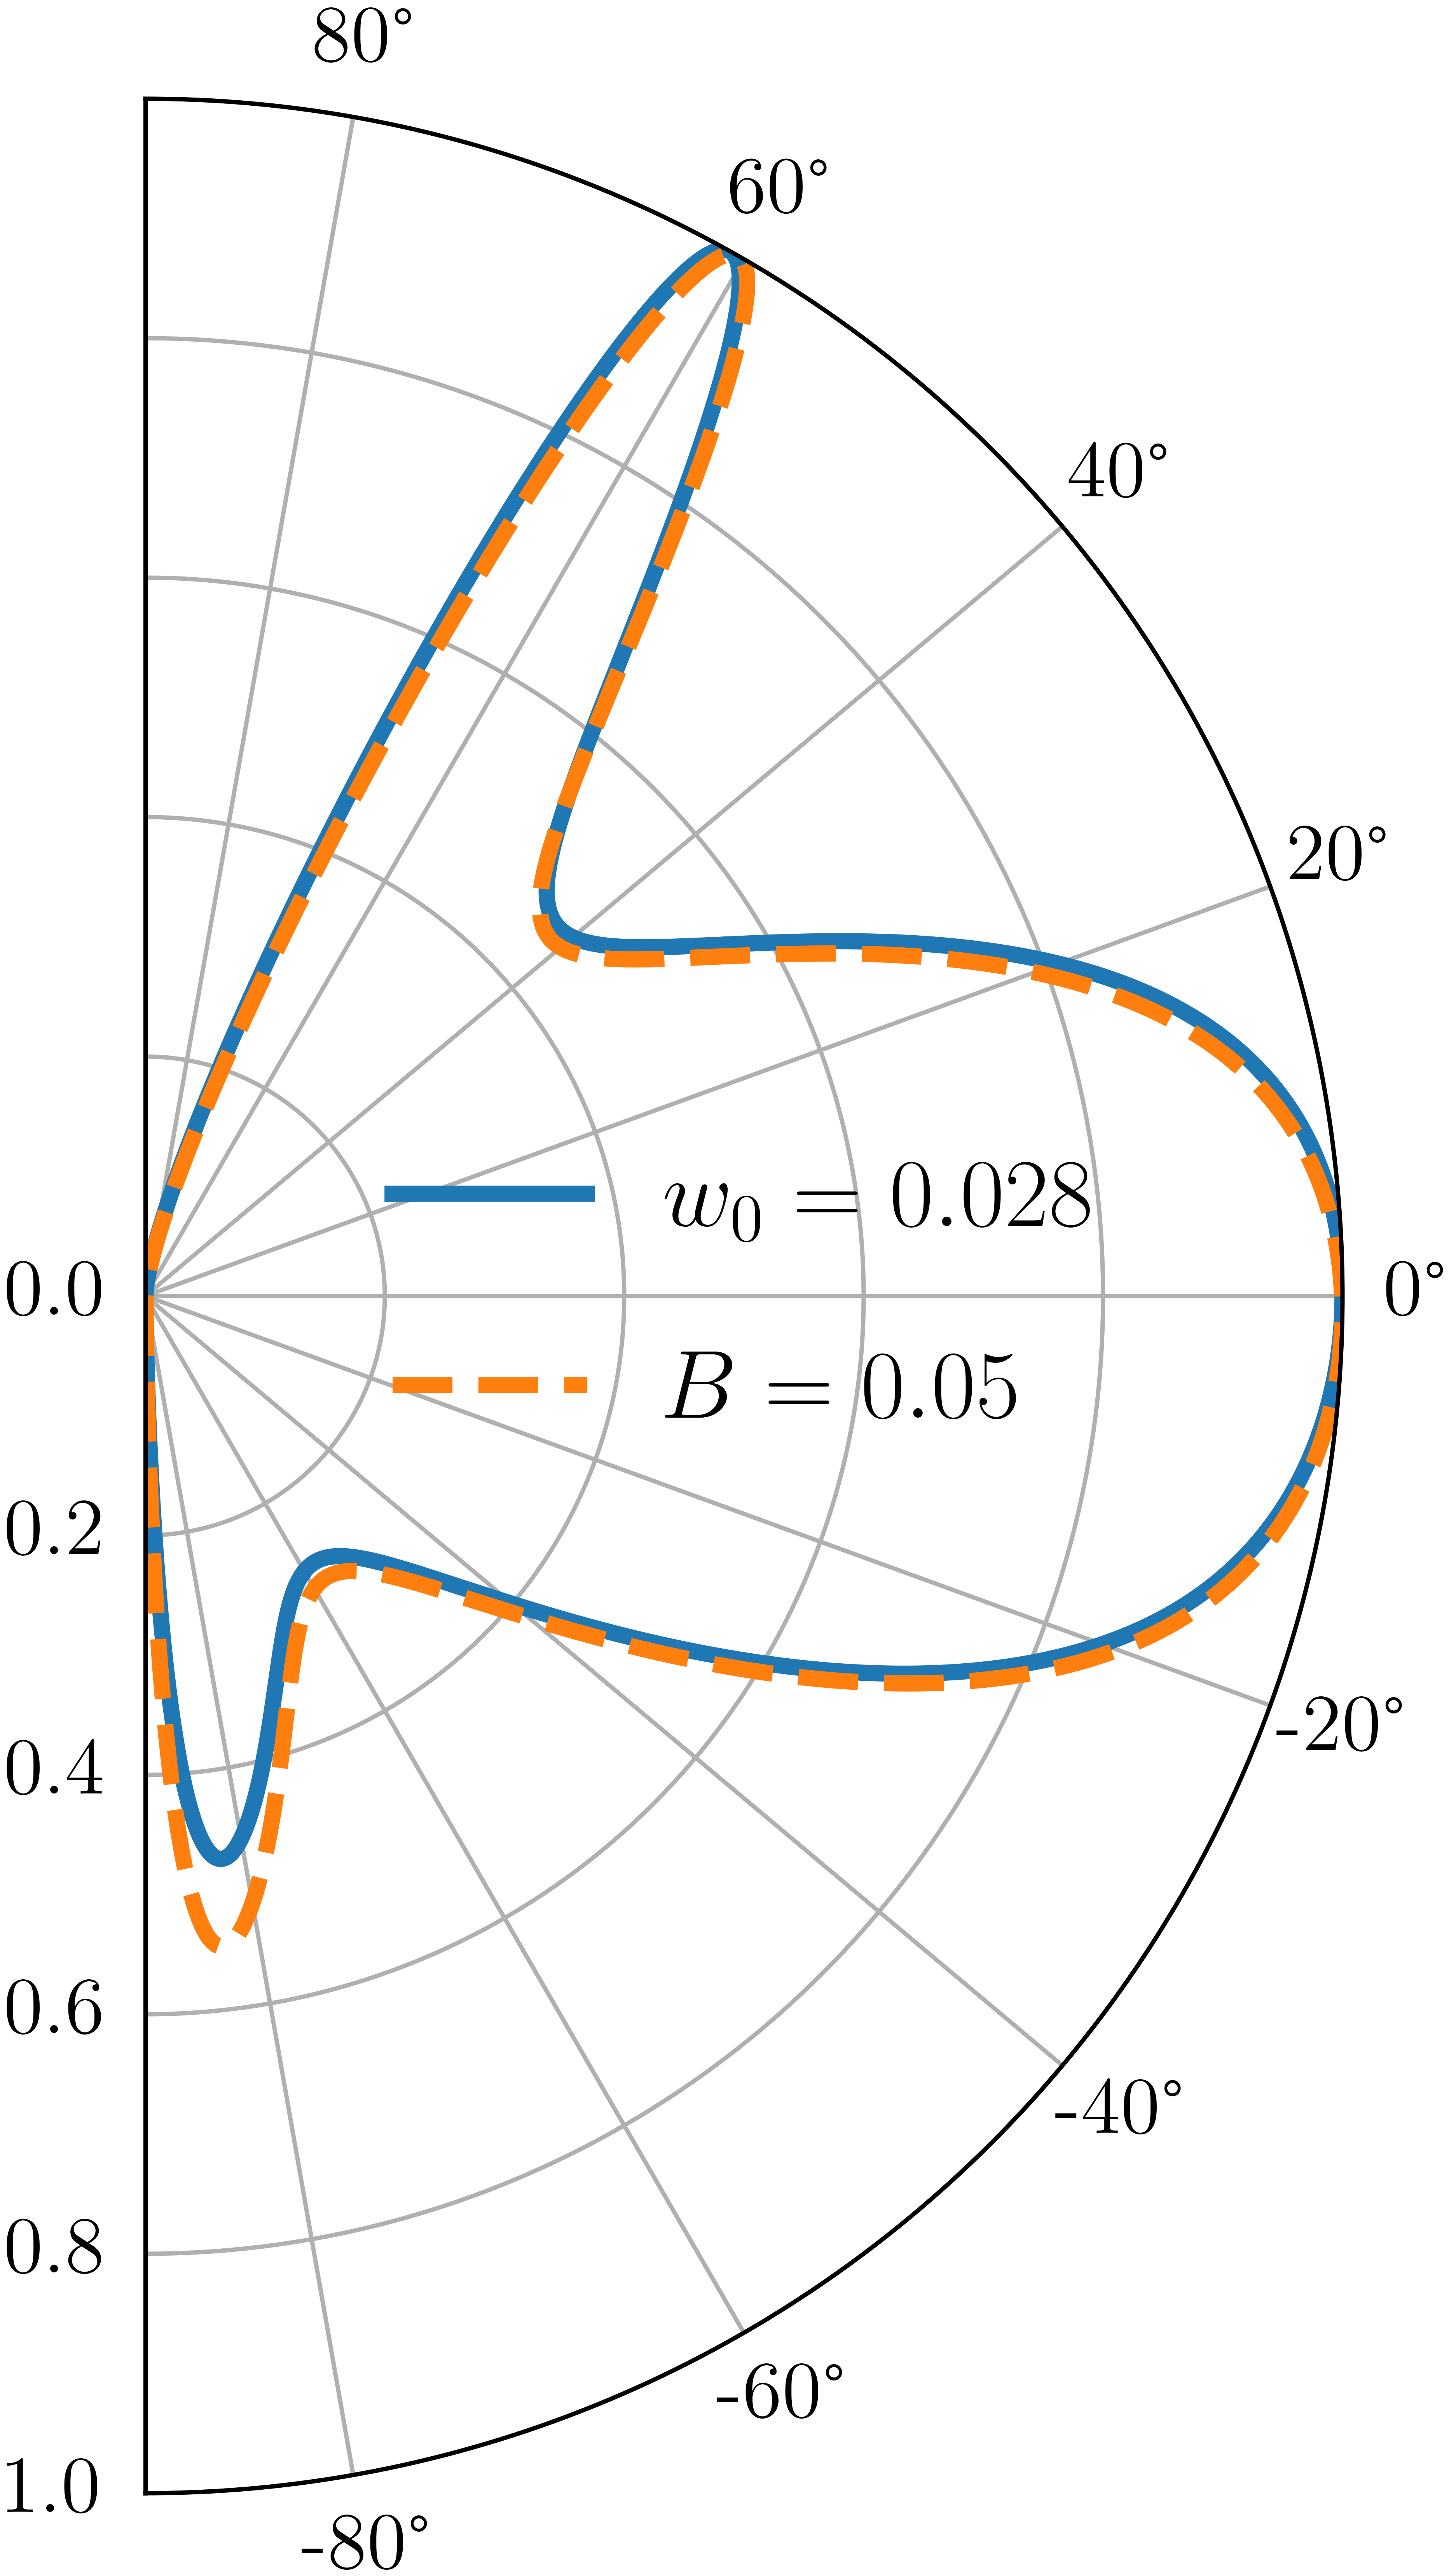
\includegraphics[width=\linewidth]{fig/pseudo B field/Ef0.0832 U0.285 B0.05 w0.028.png}
            \caption{}
            \label{fig:pseudo1}
        \end{subfigure}
        \begin{subfigure}[b]{0.3\linewidth}
            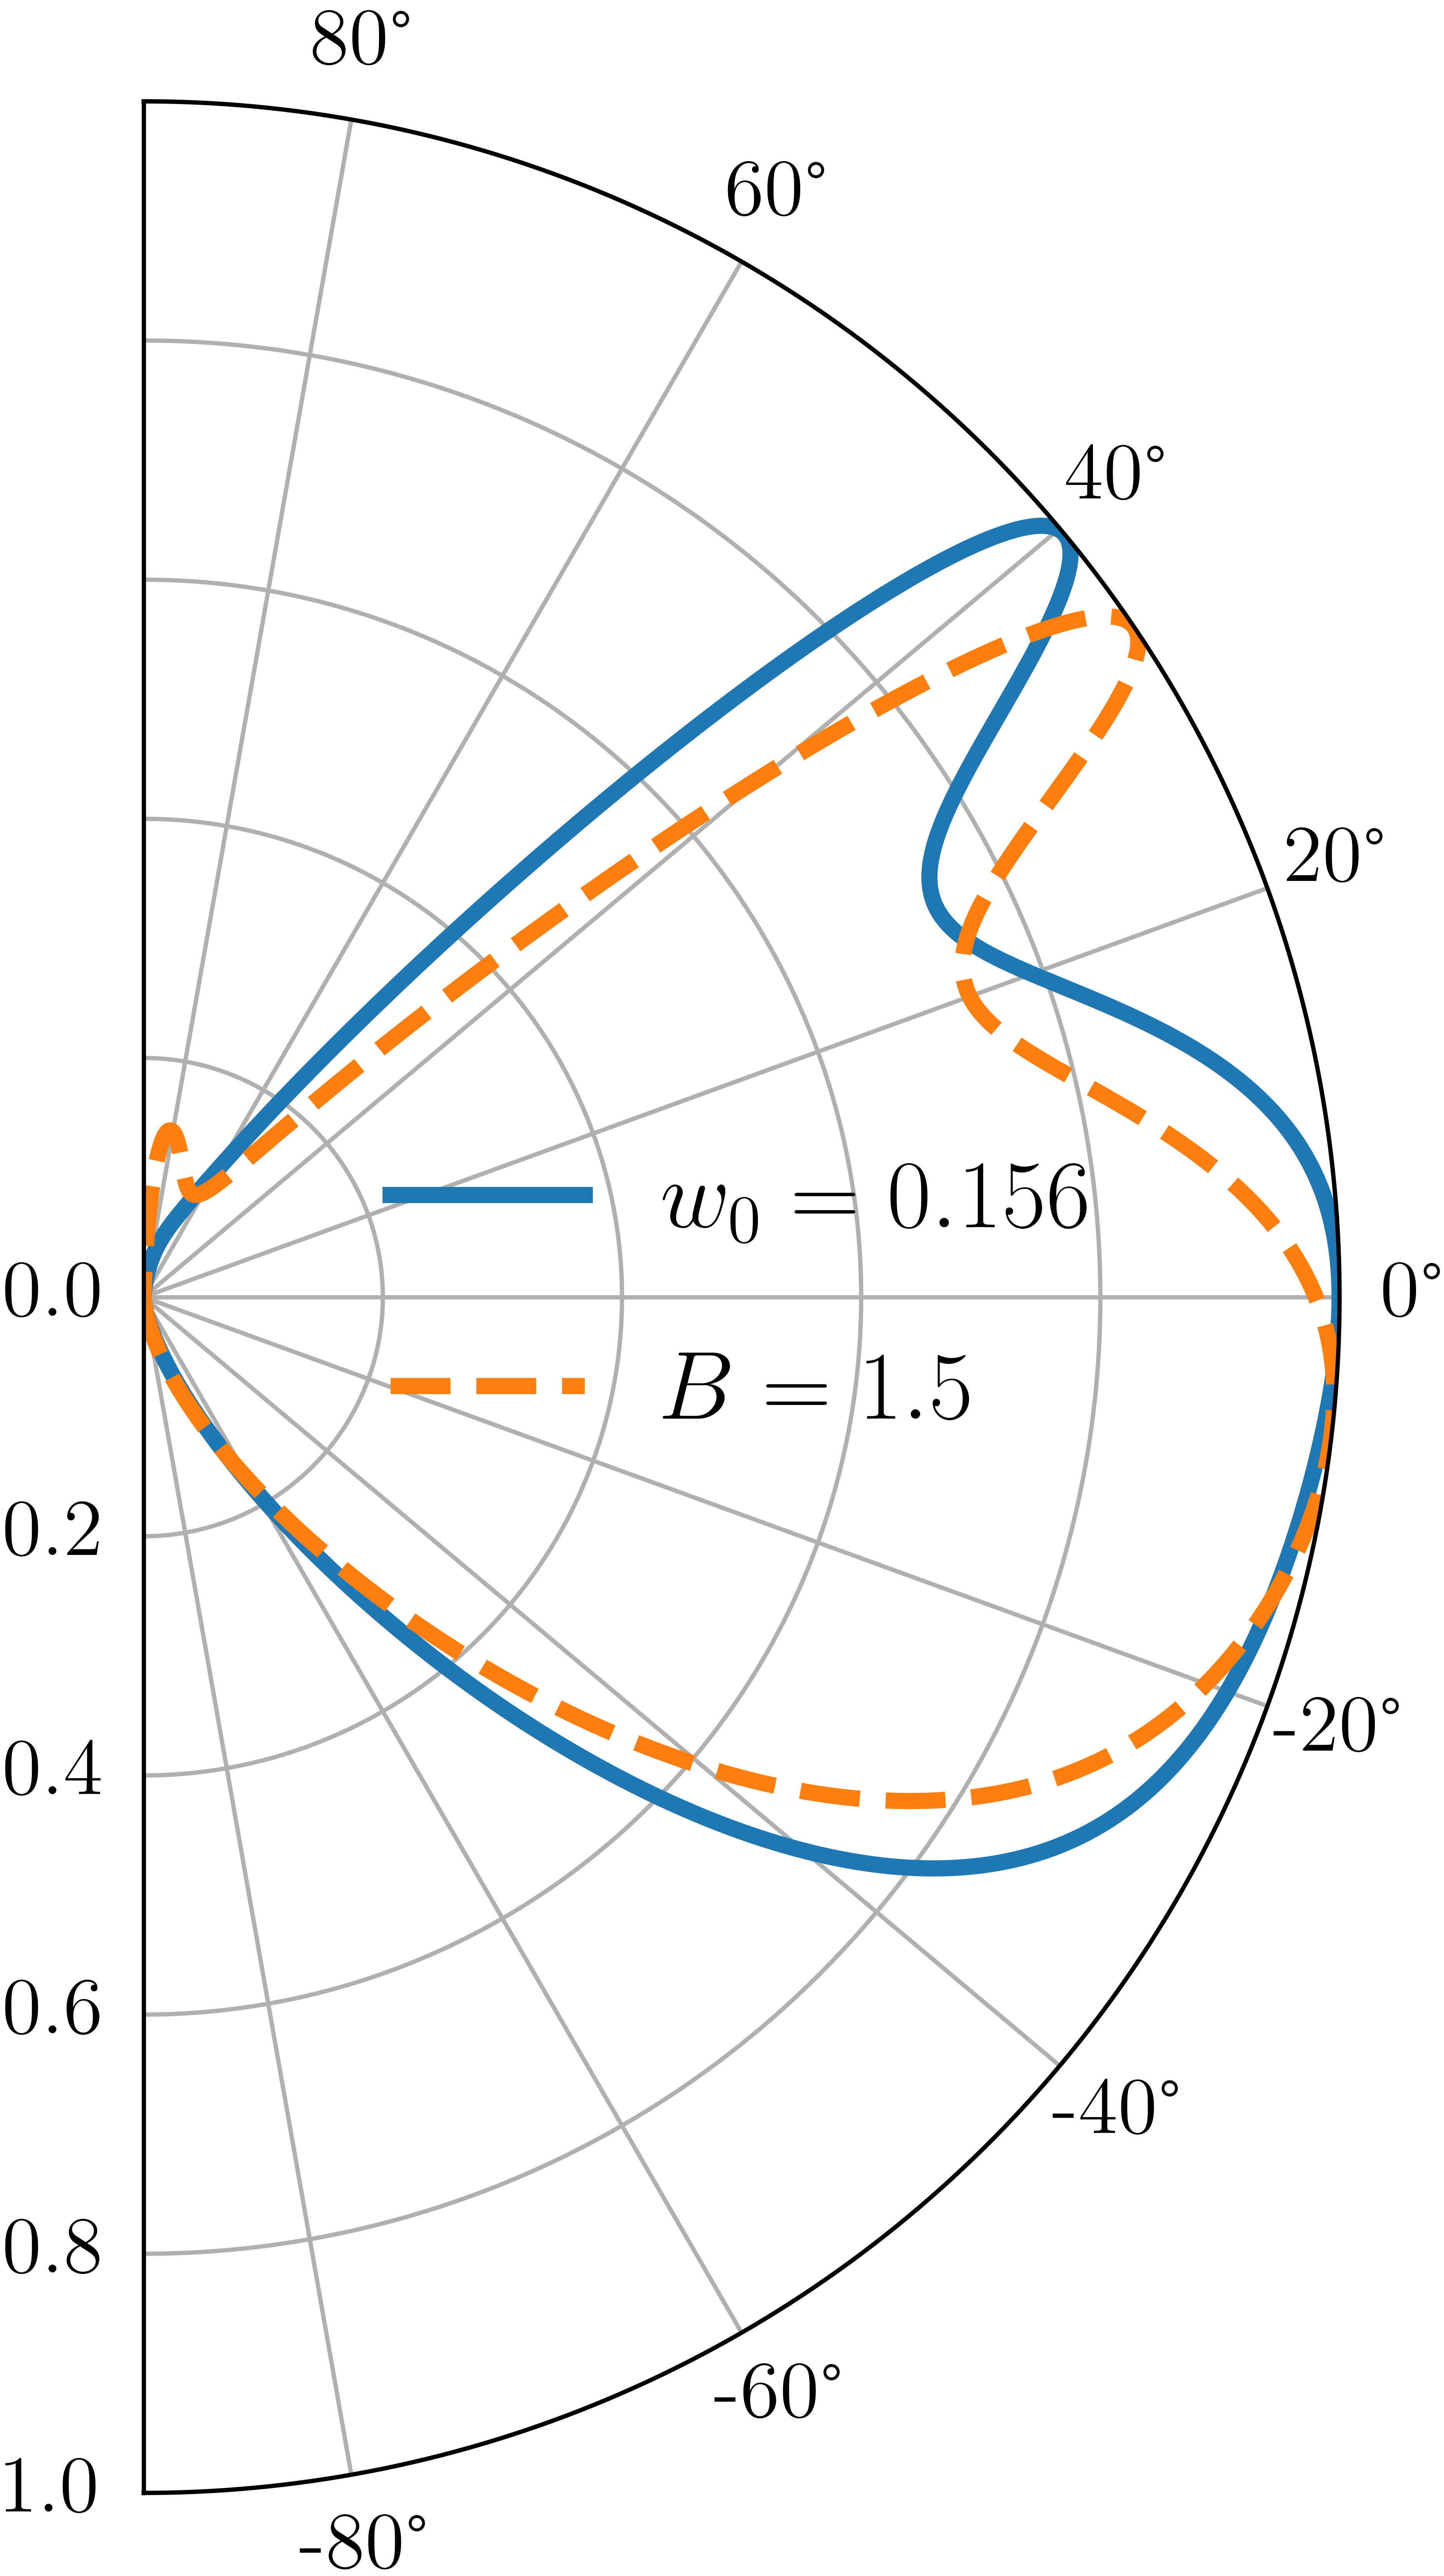
\includegraphics[width=\linewidth]{fig/pseudo B field/Ef0.0832 U0.285 B1.5 w0.156.png}
            \caption{}
            \label{fig:pseudo2}
        \end{subfigure}

        \begin{subfigure}[b]{0.3\linewidth}
            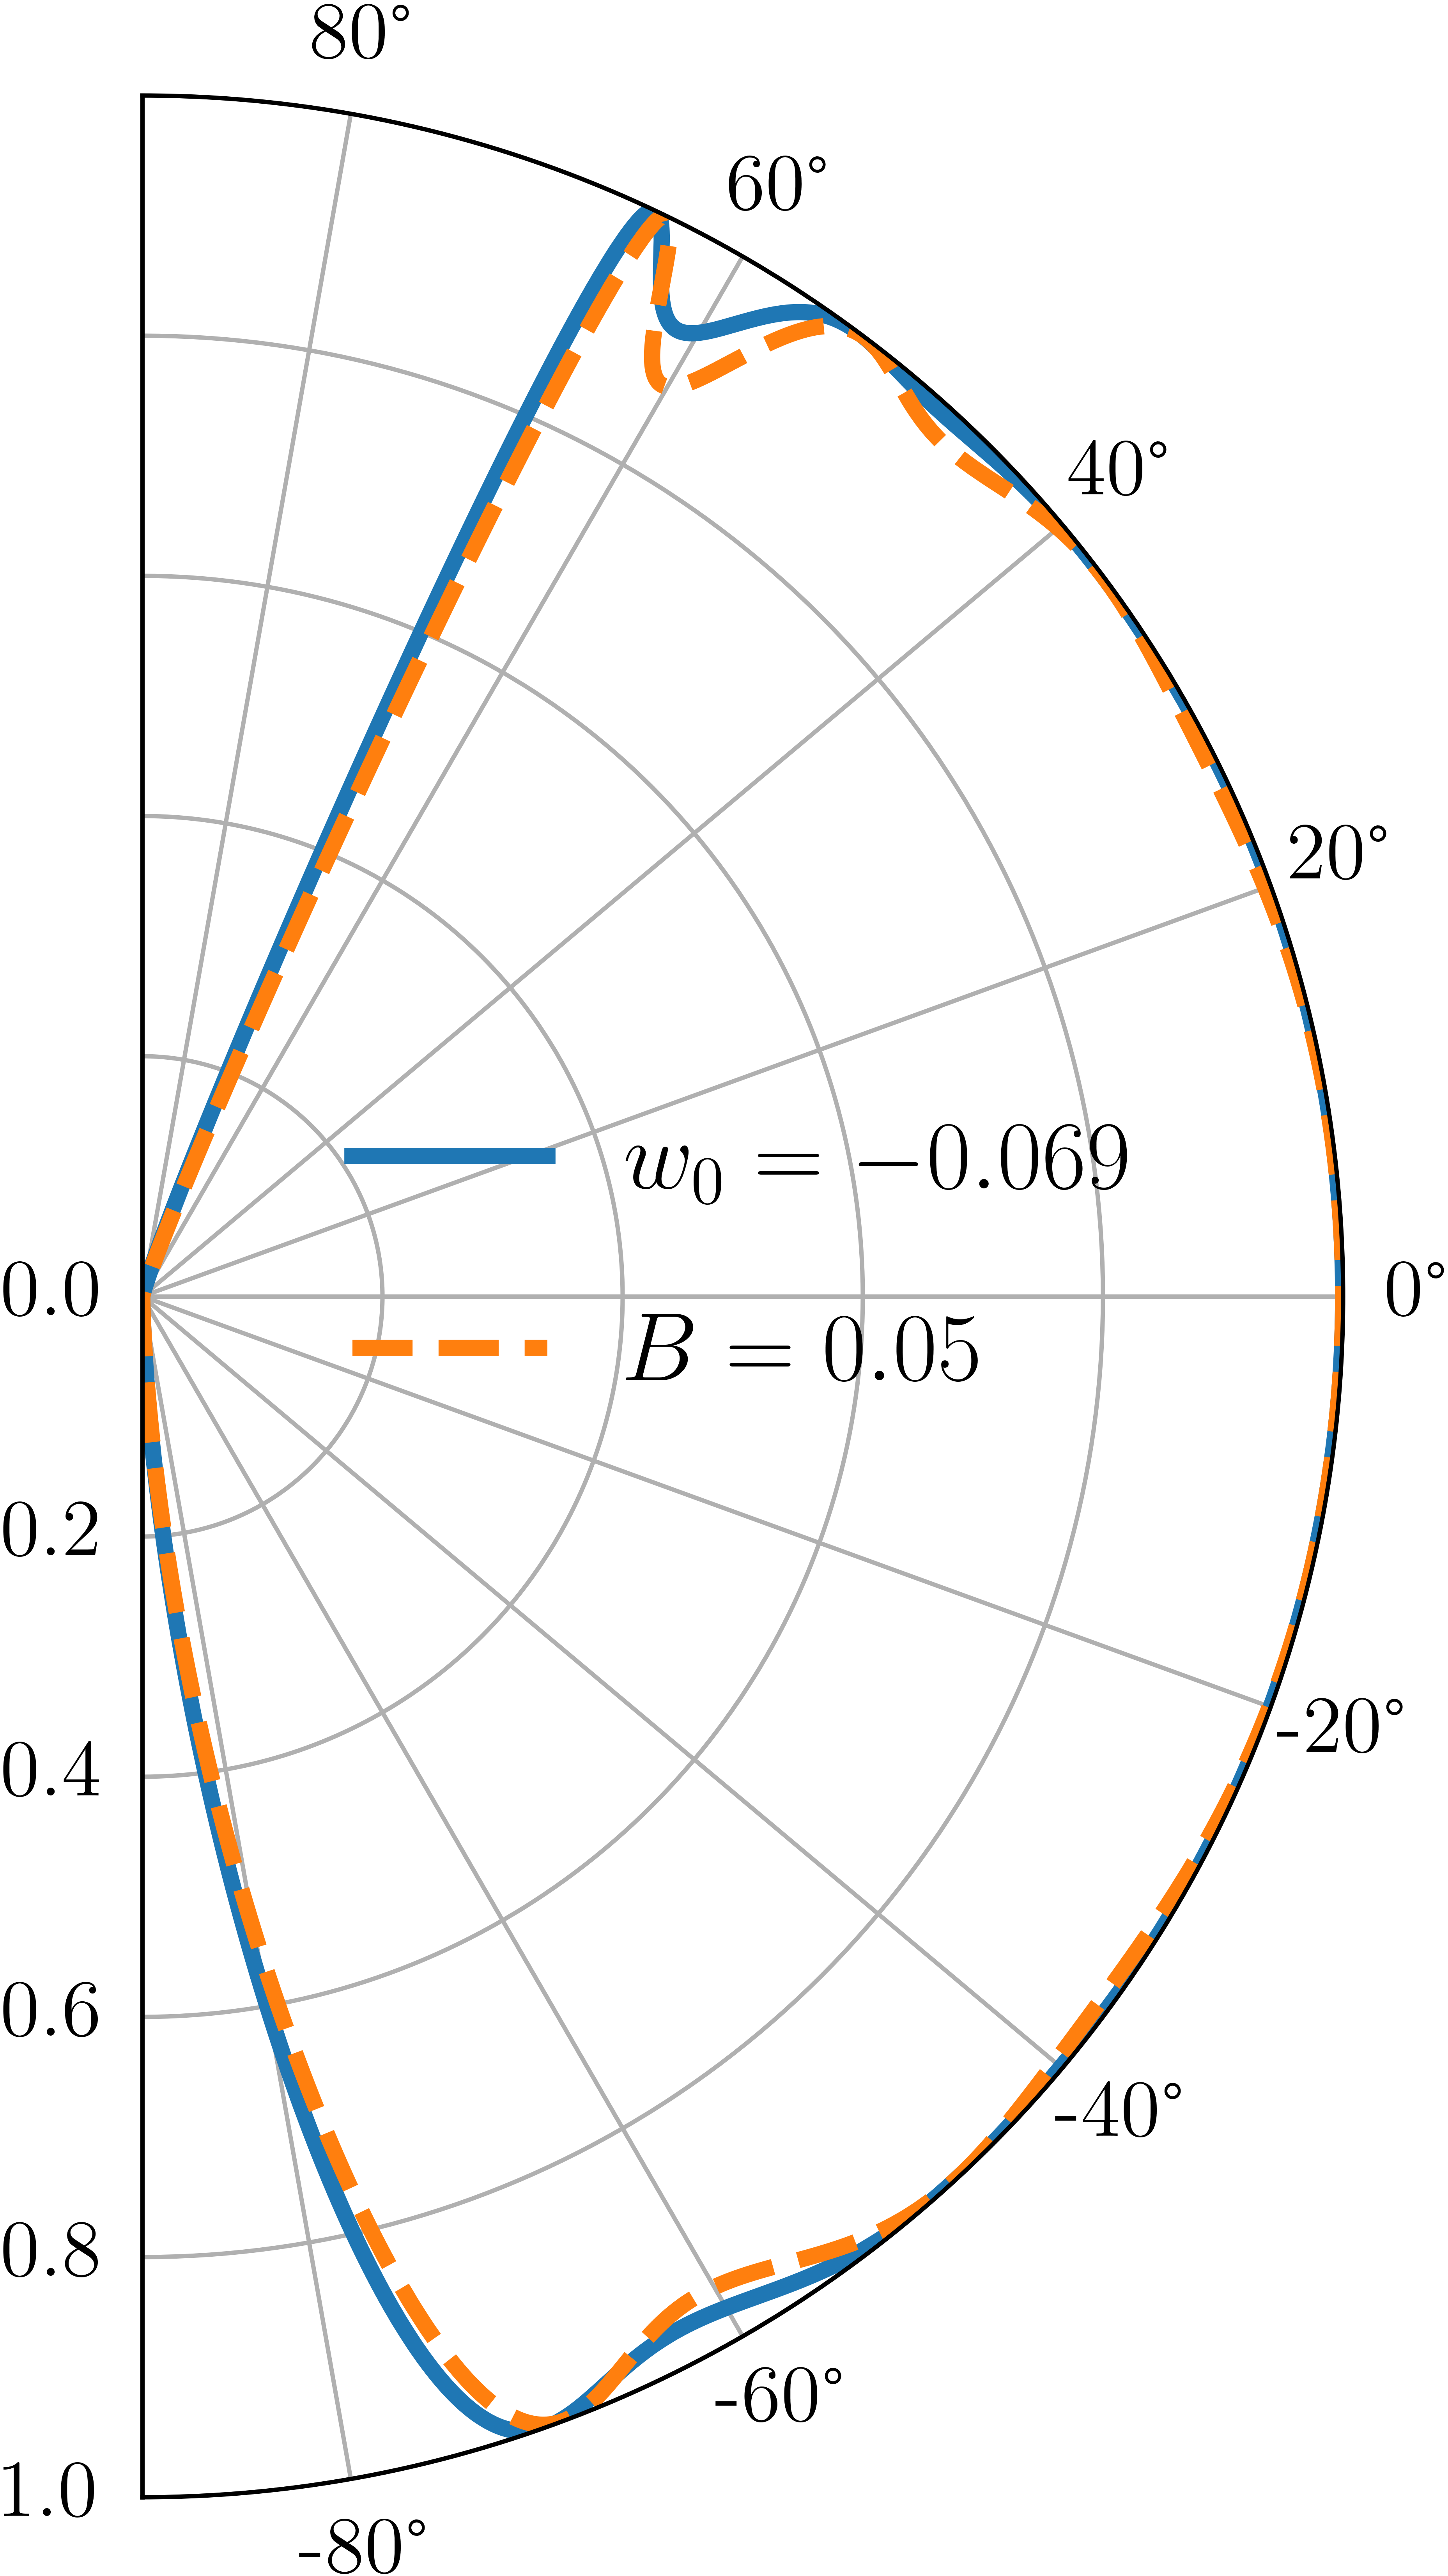
\includegraphics[width = \linewidth]{fig/pseudo B field/Ef0.0832 U0 B0.05 w-0.069.png}
            \caption{}
            \label{fig:pseudo3}
        \end{subfigure}
        \begin{subfigure}[b]{0.3\linewidth}
            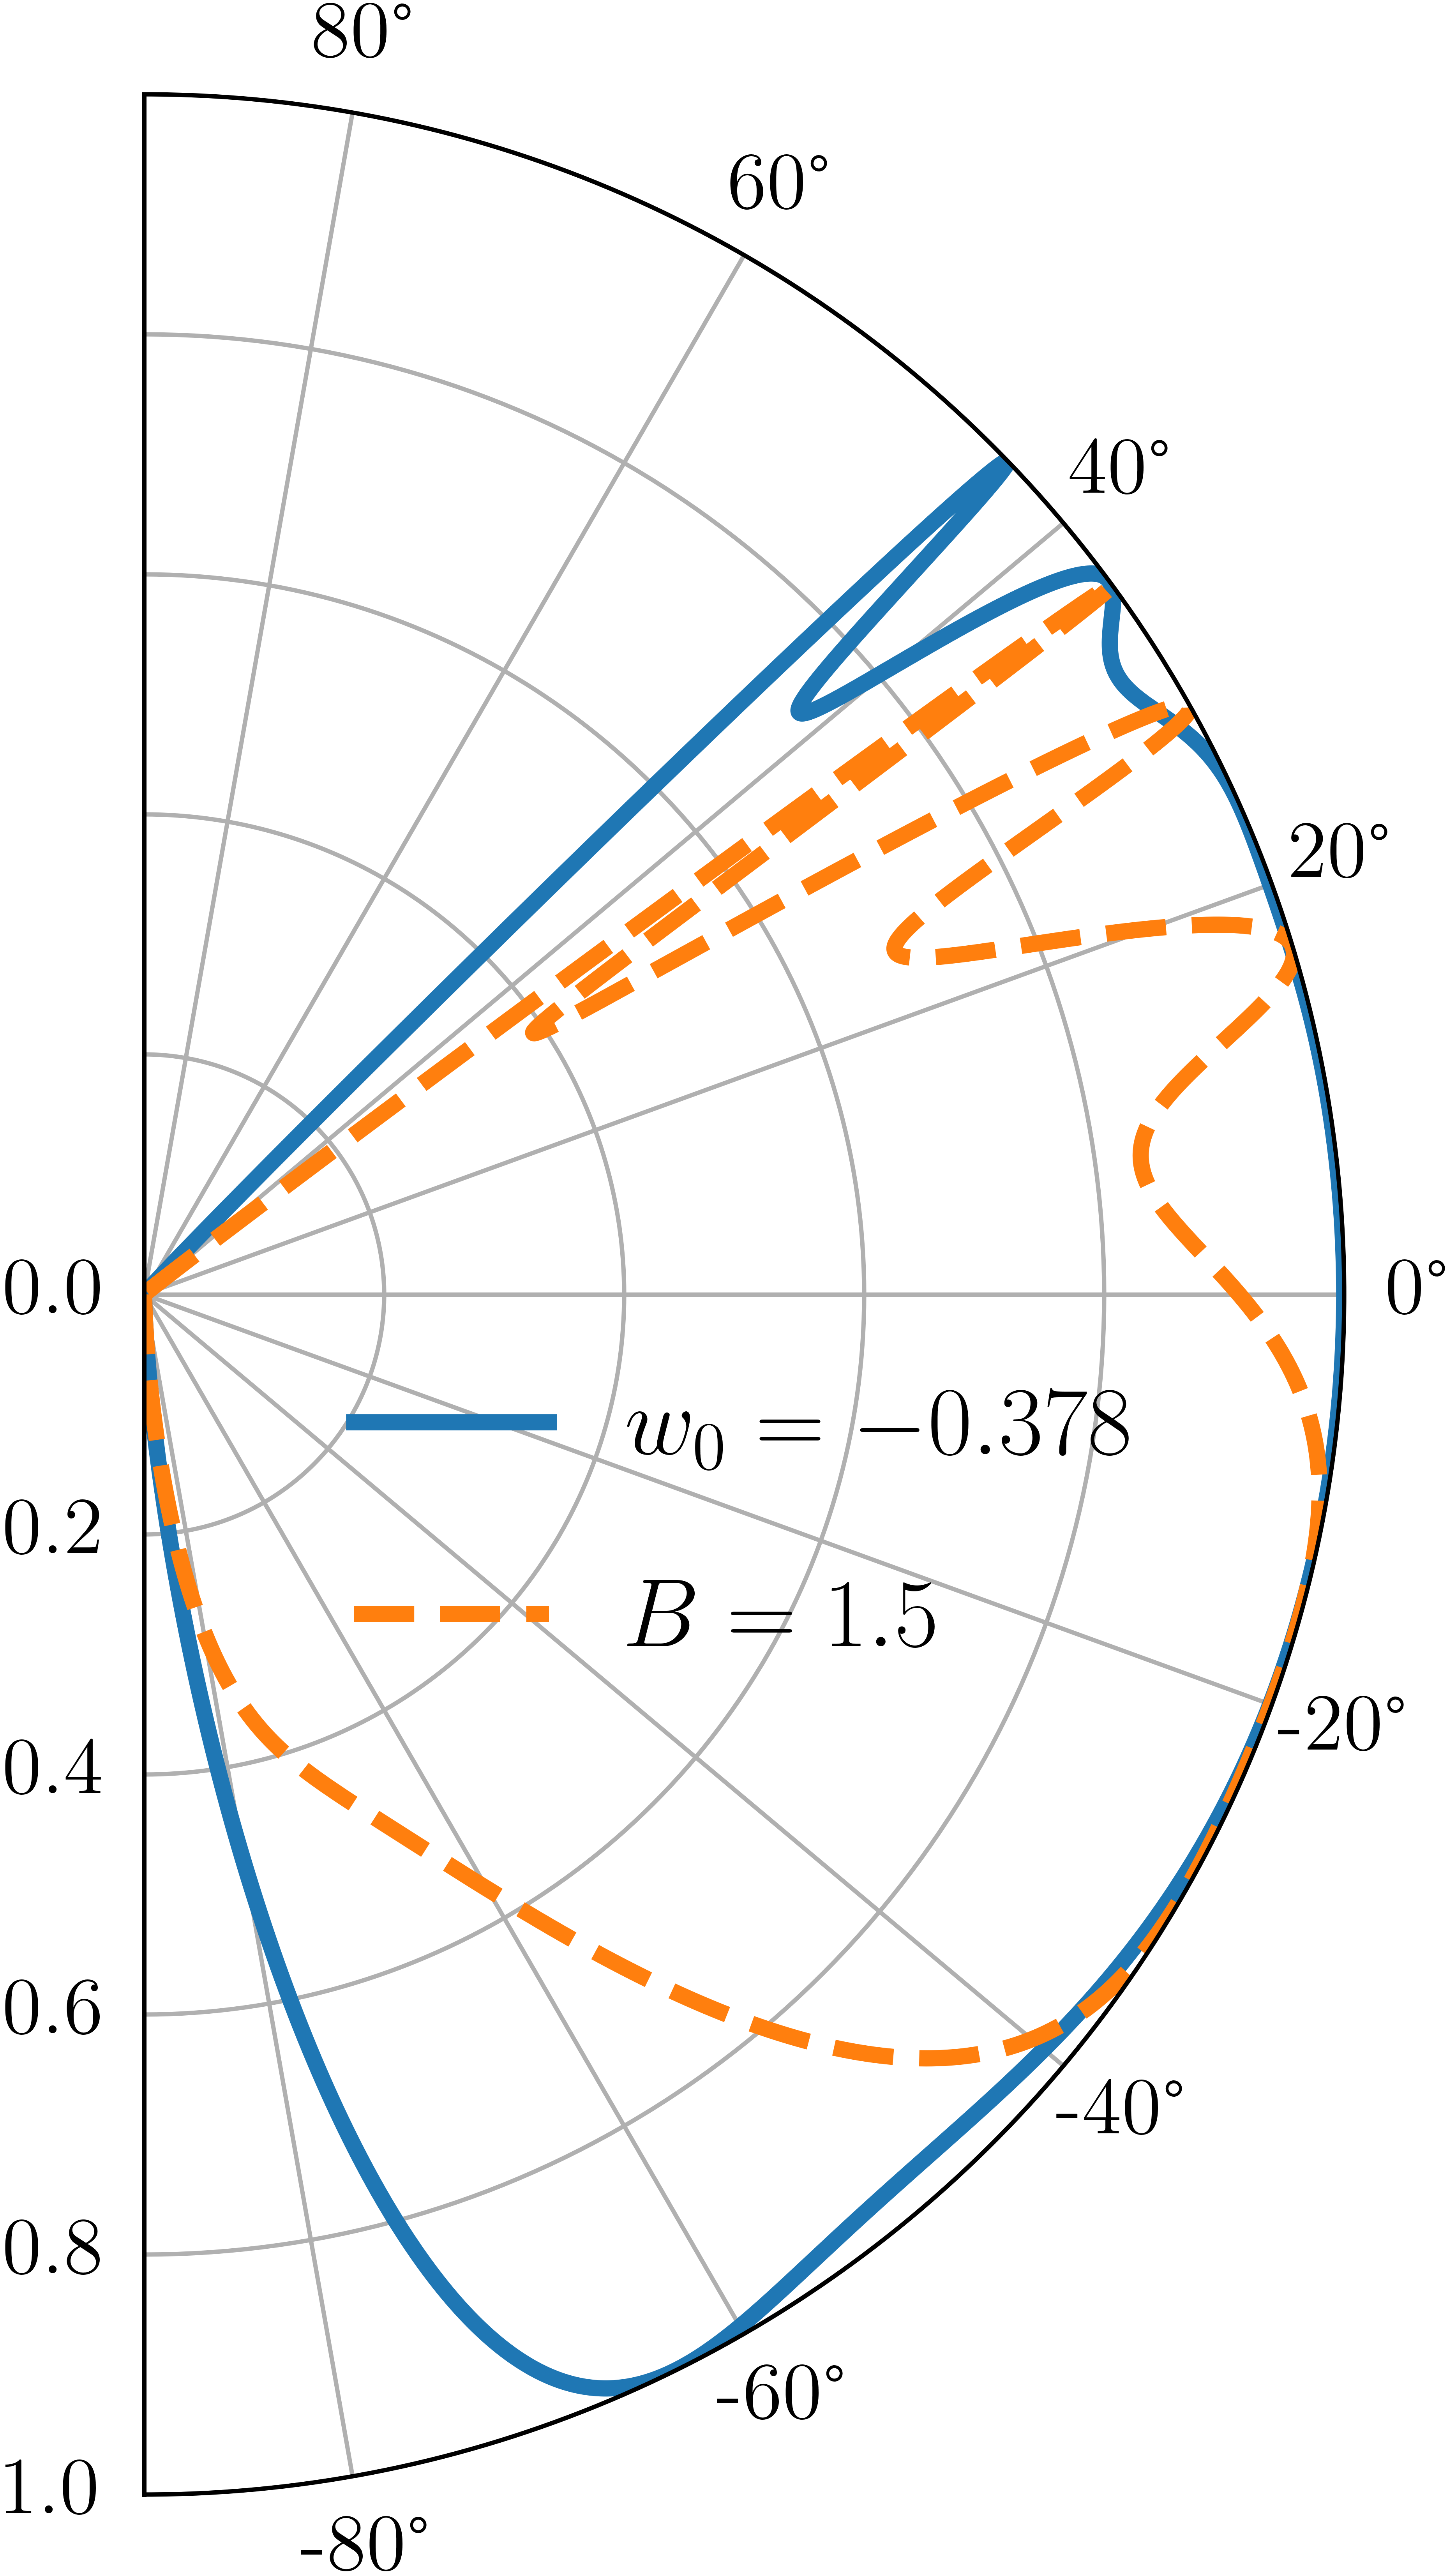
\includegraphics[width = \linewidth]{fig/pseudo B field/Ef0.0832 U0 B1.5 w-0.378.png}
            \caption{}
            \label{fig:pseudo4}
        \end{subfigure}
        \caption{The polar plot of transmission probabilities as a function of incident angle of the system with tilted mismatch Dirac cone 
                (solid line) and non-tilted system under the influence of delta magnetic field (dashed line). The Fermi energy $E_F = 83$ 
                meV is the same for all plot, the gate potential $U = 285$ meV for (a) and (b), $U = 0$ for (c) and (d) }
        \label{fig:pseudo}
    \end{figure}




    

    \kmuttchapter{CONCLUSION}
    %the effect of the tilt does not destroy the uniformity of the oscillation, it simply shifted as the tilted parameter increased.
    %The transmission probabilities of electron across tilted Dirac cone undergo the effect of pseudo magnetic field
    The observation of electronic structure has been often performed by angle-resolved photoemission spectroscopy (ARPES), which is the standard method to investigate electronic properties of material. 
    It has been suggested previously that the novel transport properties arise from anisotropy and tilt may be used to indirectly determine the character of Dirac cone \cite{Zhang2018b}. 
    Here we have shown that the asymmetric tunneling resonance can be utilized to verify the existence of the tilt. 
    By tuning the appropriate voltage at the top gate, the tilted parameter can be determined. 
    Which may be useful as an alternative method to study the electronic structure of materials. 
    We also show that the electron transport behaviors across non-tilted/tilted/non-tilted heterostructure mimic the particle under the influence of real-magnetic field in non-tilted Dirac cone system. 
    This study may be utilized for magnetic confinement applications such as magnetic waveguide. 
    This device has been previously proposed where the stripes of ferromagnetic material are used to generate the MVP barrier. 
    Which from the experimental point of view, implementing the ferromagnetic material into the device is quite challenging \cite{Awschalom2009}. 
    The pseudo-magnetic field may pave the way to design magnetic devices without magnetism. 
    \newpage

    \addcontentsline{toc}{chapter}{REFERENCES}
    %\bibliographystyle{kmutt}
    \bibliographystyle{ieeetr}
    \bibliography{library}
    \newpage

    \addcontentsline{toc}{chapter}{BIOGRAPHY}
    \kmuttchapter*{CURRICULUM VITAE}
\begin{longtable}{p{0.4\textwidth}p{0.56\textwidth}}
\textbf{NAME} & Mr. Eakkarat Pattrawutthiwong\\
\\

\textbf{DATE OF BIRTH} & 26 April  1995\\
\\

\textbf{EDUCATIONAL RECORD} & \\

HIGH SCHOOL & High School Graduation\\
            & Kaen Nakhon Wittayalai School, 2014 \\

BACHELOR'S DEGREE   & Bachelor of Science (Applied Physics) \\
                    & King Mongkut's University of Technology Thonburi, 2018 \\

MASTER'S DEGREE & Master of Science (Physics) \\
                & King Mongkut's University of Technology Thonburi, 2020 \\
\\

\textbf{SCHOLARSHIP}    & Graduated Level Scholarship, Faculty of Science, 
                        King Mongkut's University of Technology Thonburi, 2018\\
                        \\
                        &Thailand Center of Excellence in Physics Grant numbers: ThEP-61-PHM-SUT4\\
\\
\textbf{PUBLICATION}   & Soodchomshom, B., Niyomsoot, K., Pattrawutthiwong, E, 2018, 
                        "Switching effects and spin-valley Andreev resonant peak shifting in silicene superconductor," 
                        Physica E: Low-dimensional Systems and Nanostructures
                        ,Vol 97, No. 1386-9477, pp. 375-383.\\
                        \\

                        &Pattrawutthiwong, E., Choopan, W. and Liewrian, W., 2021,
                        "Possible Verification of Tilt Mismatch in Asymmetric Dirac-Cone Systems Using Resonant Tunneling Properties," 
                        Physics Letters A, Vol 393, No. 0375-9601, pp.127154.\\

\end{longtable}


\end{document}